\documentclass[a4paper]{tufte-book}
\usepackage[utf8]{inputenc}
\hypersetup{colorlinks}% uncomment this line if you prefer colored hyperlinks (e.g., for onscreen viewing)

\title{Big Data, Statistical Learning}
\author{Julien Barrier}
\publisher{ESPCI Paris}
\newcommand{\thetitle}{Introduction to Big Data}
\newcommand{\theauthor}{Julien Barrier --- class of 2018}
\newcommand{\pc}{ESPCI Paris}
\newcommand{\thesubtitle}{Statistical \& Machine Learning}

\usepackage{hyperref}
\usepackage{microtype}
\usepackage{textcase}
\usepackage{booktabs}
\usepackage{tabularx}
\newcolumntype{R}{>{\raggedleft\arraybackslash}X}

\usepackage{graphicx}
\setkeys{Gin}{width=\linewidth,totalheight=\textheight,keepaspectratio}
\graphicspath{{graphics/}}

\usepackage{fancyvrb}
\fvset{fontsize=\normalsize}

\newcommand{\hangp}[1]{\makebox[0pt][r]{(}#1\makebox[0pt][l]{)}}

\newcommand{\hangstar}{\makebox[0pt][l]{*}}

\usepackage{xspace}

\newcommand{\monthyear}{%
\ifcase\month\or January\or February\or March\or April\or May\or June\or
July\or August\or September\or October\or November\or
December\fi\space\number\year
}

\newcommand{\openepigraph}[2]{%
%\sffamily\fontsize{14}{16}\selectfont
\begin{fullwidth}
\sffamily\large
\begin{doublespace}
\noindent\allcaps{#1}\\% epigraph
\noindent\allcaps{#2}% author
\end{doublespace}
\end{fullwidth}
}

\newcommand{\blankpage}{\newpage\hbox{}\thispagestyle{empty}\newpage}

\usepackage{units}
\usepackage{siunitx}
\usepackage{stmaryrd}
\usepackage{amsmath,amsfonts,amssymb}
\usepackage{mathrsfs}
\usepackage{dsfont}
\newcommand{\measure}[3]{#1/#2$\times$\unit[#3]{pc}}
\DeclareMathOperator{\sign}{sign}

\newcommand{\hlred}[1]{\textcolor{Maroon}{#1}}% prints in red
\newcommand{\hangleft}[1]{\makebox[0pt][r]{#1}}
\newcommand{\hairsp}{\hspace{1pt}}% hair space
\newcommand{\hquad}{\hskip0.5em\relax}% half quad space
\newcommand{\TODO}{\textcolor{red}{\bf TODO!}\xspace}
\newcommand{\ie}{\textit{i.\hairsp{}e.}\xspace}
\newcommand{\eg}{\textit{e.\hairsp{}g.}\xspace}
\newcommand{\na}{\quad--}% used in tables for N/A cells
\newcommand{\E}{\mathrm{E}}
\newcommand{\var}{\mathrm{Var}}
\newcommand{\cov}{\mathrm{Cov}}
\newcommand{\half}{\frac{1}{2}}
\newcommand{\nth}{\frac{1}{N}}
\newcommand{\sumin}{\sum_{i=1}^N}

% Generates the index
\usepackage{makeidx}
\makeindex

\usepackage{titlesec,titletoc}
\usepackage{multirow}

\begin{document}
\frontmatter

\thispagestyle{empty}
\begin{fullwidth}
    \setlength{\parindent}{0pt}
    \begin{center}
        \fontsize{24}{24}\selectfont\textit{
            \includegraphics*[width=2.6in]{ESPCI_baseline_couleur}
        }
    \end{center}
    \vspace{3in}\fontsize{36}{54}\selectfont\thetitle

    \vspace{0.125in}\fontsize{18}{18}\selectfont\thesubtitle

    \vfill\fontsize{14}{14}\selectfont\textit{\theauthor}
\end{fullwidth}

\newpage

\cleardoublepage
\chapter*{Introduction}

I have started writing this handout from the notes I have taken from
Olivier Rivoire's course on Big Data and Statistical learning at \pc{} from
March to April 2018. The \LaTeX ~sources of this document can be found on
\href{https://github.com/julienbarrier/bigdata-handout}{Github}. Do not hesitate
to update it if you feel it necessary.

Please be considerate if some mistakes crop up in this work.

\vspace{.5cm}
\emph{Julien}
\vspace{1cm}

Some book reading is advised during the course, partialicularly:

\begin{itemize}
    \item \emph{The Elements of Statistical Learning}, T.~Hastie, R.~Tibshirani and J.~Friedman, Springer Series in Statistics, 2008;
    \item \emph{Information Theory, Inference, and Learning Algorithms}, D.J.C.~MacKay, Cambridge University Press, 2003.
\end{itemize}

\vspace{1cm}

\textbf{Dr Olivier Rivoire}\\
Center for Interdisciplinary Research in Biology (CIRB)\\
Collège de France\\
olivier.rivoire@college-de-france.fr\\

\section*{Applications}

There are plenty of applications for Big Data problems. A few examples may be
given:
\begin{description}
    \item[Post] learn + identify digits on enveloppes
    \item[Biology] DNA sequencing
    \item[IT] Face recognition
    \item[etc.]
\end{description}

Big Data is an issue of growing importance. As engineers, we may be familiar 
with such concepts.
 \section*{Idea of marchine learning} 

The main idea of machine learning is to find models to give prediction of input data.
In facts, Big Data models are deduced from a training batch of N input-output
data, on which programs train to generalise models.
The deduced model \emph{input i} $\rightarrow$ \emph{output i} can then be
generalised to give prediction from a random input, as long as it relates to 
the training batch.



Analytically, let's start with a collection of $x$ and $y$ data, where $x$ 
stands for the input data and $y$ is the vector of the output data.
Each sample is going to have multiple dimensions, therefore we may use an
algebraic model. Let $N$ be the number of samples used and p the dimension of
each $x$ data. We may write x as an $N,p$ matrix and $y$ as a vector of $p$
dimensions.

We now N samples of p dimensions $x_{ij}$ associated with the N output data
$y_i$.

From now on there are two possible cases: $y_i$ can be known or unknown.
In the fist case ($y_i$ known), the problem is said to be \emph{supervised}.
Hence we may work with a finite discrete set of data: $y_i = 1, \cdots, K$.
This problem is called categorical, and we can solve it with 
\emph{classification}.
We may also work with an infinite set of numbers: $y_i \in \mathbb{R}$. This
problem is called quantitative, and we can solve it with \emph{regression}.

The second case ($y_i$ unknown) is said to be \emph{unsupervised} and can be
solved via \emph{clustering} or \emph{dimension reduction} methods.

\section*{Deep learning}

In the past few years, there have been huge progress in the \emph{deep learning}
approach. It is based on so-called neural networks, that are models inspired
by the brain operation.

People are trying to understand how to train these networks. It has had
remarkable outcomes in image recognition, social network filtering, medical
diagnoses, etc.

Deep learning is based on hidden layers, placed inbetween input and output
layers, that are trained to find correlations and mathematical models.

The goal of this course is to explain whate these objects are, how do they work,
and put it in relation with state of the art research.

What kind of open problems are there? How do neural networks operate? What are
their unsuperised learning behaviour?


\tableofcontents\thispagestyle{empty}

\mainmatter

\chapter{Least square regression, from small to big data}
\label{ch:least-square}

\section{Linear Regression at One Dimension}

Let us work at one dimension: $p =1$. If we work with N points, then
$i=1,\cdots,N$, and we work with a set of data $(x_i,y_i)$.

The goal here is to make a prediction of what the $y$ data should be when $x$ is
given.

The simplest possible model is the linear regression given by the equation 
\ref{linear1D}.

\begin{equation}
    y=\alpha + \beta x.
    \label{linear1D}
\end{equation}
Here, the main issue is to get the best $\alpha$ and $\beta$ for a partialicular
set of data. To know what the best choice is, we may define a cost function,
that returns a number representing how well the regression permorms. In neural
network problems, the cost fuction return number is associated with how well the
neural network performs in mapping training examples to the correct output.

There are several choices that can be made to define the cost function. At one
dimension, the simplest choice is the sum of squared residuals, defined in
equation \ref{SSR}, usually shortened as SSR.

\begin{equation}
    l(\alpha,\beta) = \nth \sumin (y_i - \alpha - \beta x_i )^2
    \label{SSR}
\end{equation} 

Figure \ref{fig1} illustrate a simple geometrical interpretation of what the SSR
is. Actually, the lower $\epsilon_i$, the better the fit.

\begin{marginfigure}
    \TODO
    \caption{geometrical intepretation of the SSR, where $\epsilon_i$ is given
        by the relation: $\epsilon_i^2 = (y_i - \alpha - \beta x_i)^2$}
    \label{fig1}
\end{marginfigure}

For all we have done up to now, we never have never worked with big data. We
need $p$ large enough to consider this as a real big data issue.

If we’re looking at a hundreds or thousands pixels picture, $p$ will be large
in comparison with $N$. That is a full statistics problem.

Currently, $p=1$ is small data, but all we did there has been a correct
introduction to clearly understand big data problems.

Striking a good fit necessitates finding the best $\alpha$ and the best $\beta$.
For this, we may look at the optimum, defined as the points where the derivative
of $l$ versus $\alpha$ and $\beta$ vanishes. This is given by equations
\ref{derlalpha} and \ref{derlbeta}.

\begin{eqnarray}
    \frac{\partial l}{\partial \alpha} & = & - \nth\sumin (y_i - \alpha - \beta x_i) = 0
    \label{derlalpha}\\
    \frac{\partial l}{\partial \beta} & =&  -\nth\sumin  x_i (y_i - \alpha -  \beta x_i) = 0
    \label{derlbeta}
\end{eqnarray}

To solve this set of equations, we require a substitution for $x$ and $y$.

Let’s define the mean values:
\marginnote{We must keep in mind that $\overline{x^2} \neq \bar{x}^2$.}
\begin{eqnarray}
    \bar{x} & = & \nth\sumin x_i\\
    \bar{y} & = & \frac{1}{N} \sum_{i=1}^N y_i\\
    \overline{xy} & =&  \frac{1}{N} \sum_{i=1}^{N} x_i y_i\\
    \overline{x^2} & =&  \frac{1}{N} \sum_{i=1}^N x_i^2
\end{eqnarray}

Thus, equations \ref{derlalpha} and \ref{derlbeta} can be reduced as:
\begin{eqnarray}
    \frac{\partial l}{\partial \alpha} &=& - (\bar{y} - \alpha - \beta \bar{x})
    \label{deralpha2}\\
    \frac{\partial l}{\partial \beta} &=& - (\overline{xy} - \alpha \bar{x} - \beta \overline{x^2})
    \label{derbeta2}
\end{eqnarray}

This yields to:

\begin{eqnarray}
    \alpha & = & \bar{y} + \beta \bar{x}\\
    \overline{xy} & = &  -\bar{y}\bar{x} - \beta \bar{x}^2 - \beta \overline{x^2}
\end{eqnarray}

\marginnote{We use the given notations:
    \begin{eqnarray*}
        \cov(x,y) &=& \bar{xy} - \bar{x}\bar{y} \\
        & =& \overline{(x-\bar{x})}(y-\bar{y}) \\
        \var(x) & =&  \cov (x,x) \\
        \sigma(x) & =& \sqrt{\var(x)}
    \end{eqnarray*}
}

There we may substitute $\alpha$ and $\beta$:

\begin{eqnarray*}
    \hat{\alpha} & =& \bar{y} - \hat{\beta}\bar{x}
\end{eqnarray*}

\begin{eqnarray*}
    \hat{\beta} & = & \frac{\overline{xy} - \bar{x}\bar{y}}{\overline{x^2} - \bar{x}^2} \\
    & = & \frac{\cov(x,y)}{\cov(x,x)}\\
    & =&  \frac{\cov(x,y)}{\var(x)}
\end{eqnarray*}


Let us define the Pearson coefficient $\mathcal{R}$ by the relation
\ref{pearson}.
\begin{equation}
    \mathcal{R} = \frac{\cov(x,y)}{\sigma(x) \sigma(y)}
    \label{pearson}
\end{equation}

The Pearson coefficient $\mathcal{R}$ is always comprised between $0$ and $1$.
Thus, we can define the quantity $\mathcal{R}^2$, that relates to the quality of
the fit:

\begin{equation}
    \mathcal{R}^2 = 1 - \frac{\hat{l}}{\var(y)}
\end{equation}


In the general case, we look at models where $\beta = 0$. In this case, the cost
function $l$ would be the sum of the square distance to the line.
Figure \ref{squaredistances} depicts two linear regressions with different
parameters. The right figure shows a much better linear regression, with
much lower square distances between the points and the line.

\begin{figure}
    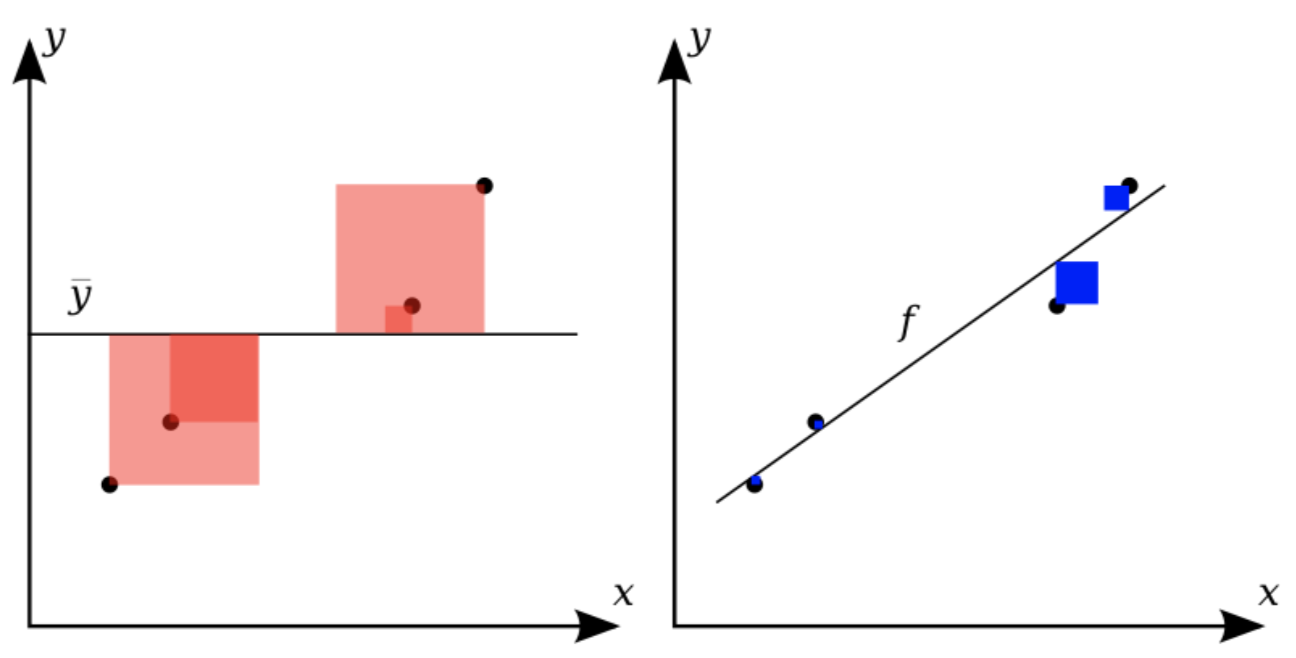
\includegraphics{./Figures/squaredistances.png}
    \caption{Two linear regression taken from two datasets. The left one shows higher square distances than the right one.}
    \label{squaredistances}
\end{figure}

We may note that in some cases, it would be better to rescale the axis to
fit the data with a linear regression. Logarithm axis is the most popular way
of rescaling an axis to have a correct assumption. It is usually more valuable
to rescale the axis and perform a linear regression, than trying to find an
higher order fit.

\section{Linear Regression at Higher Dimensions}

We are now considering higher dimensions data ($p>1$), that are full, meaning
that $p<<N$.
It means that, for an example of data, we might add different parameters. If we
take the example (given in class) of correlations between the velocity of people
versus the size of towns, we might add other relevant parameters, like the
average heigh of people, their ages, etc. We might then examine many potential
predictors. Thus we need to generalise the same things, where each input now
becomes a vector of p dimensions, as presented in equation \ref{pdim}

\begin{equation}
    (x_{i,1}, \cdots , x_{i,p}), \qquad \forall i
    \label{pdim}
\end{equation}

Let now $x_{i,j}$ be the matrix of the input data, where $i$ is the number of
samples, varying from 1 to $N$, and $j$ is the dimension, ranged between 1 to
$p$.

We may generalise the relation $\hat{y_i} = \hat{\alpha} + \hat{\beta}x_i$ in
the new \ref{gen2} equation: 

\begin{equation} 
    \hat{y_i} = \hat{\alpha} + \sum_{j=1}^p \hat{\beta_j} x_{ij}
    \label{gen2}
\end{equation}

If we have this key figure, we can always add 1 in the x vector, as the $p+1$
coordinate. We can thus assume that $\alpha$ vanishes. In fact, we can always
redefine the data so that $\alpha$ vanishes. We can also rescale the variable, by
removing the mean:

\begin{eqnarray}
x’&=& x-\bar{x}\\
y’&=& y-\bar{y}
\end{eqnarray}

Therefore, the output coordinate $\hat{y_i}$ can be written as the product
$\hat{y_i} = X \hat{\beta}$, that is a much more convenient way to write it.

That are just restrictions of the problems that help us to compute it.

Let $l(\beta)$ be the cross-function, define with equation \ref{lbeta}.

\begin{equation}
    l(\beta) = \frac{1}{N} \sum_{i=1}^N \left( y_i - \sum_{j=1}^p \beta_j x_{ij} \right)^2
    \label{lbeta}
\end{equation}

\marginnote{$^T$ denotes the transpose matrix, defined by the relation:
$\left[\mathbf{A}^\mathrm{T}\right]_{ij} = \left[\mathbf{A}\right]_{ji}$}

Let $Z$ be a vector whose components $z_i$ are defined as follows:

\begin{equation}
    \sum_{i=1}^N z_i^2 = ||Z||^2 = Z^TZ
\end{equation}

Therefore we can write the cross-function as:

\begin{equation}
    l(\beta) = \frac{1}{N} (Y-X\beta)^T(Y-X\beta)
\end{equation}

This form can easily be differentiated with $\beta$, and the retrieved derivative
vanishes at the extremum (eq. \ref{lextrem}).

\begin{equation}
    \frac{\partial l}{\partial \beta} =  -\frac{Z}{N} X^T(Y-X\beta) =0
    \label{lextrem}
\end{equation}

The equation \ref{lextrem} can be reduced as $X^TY = X^TX\beta$, which can be
solved by introducing the matrix $C = X^TX$ (eq. \ref{lextremC})\footnote{Note
    that 
\begin{equation*}
C_{ij} = \sum_{k=1}^N x_{kj} x_{ki}
\end{equation*}}

\begin{equation}
    \hat{\beta} = (X^TX)^{-1} X^TY = C^{-1} X^TY
    \label{lextremC}
\end{equation}

At higher dimension, the geometry consists in fitting with an hyperplane, as
shown on figure \ref{hyperplane}.

\begin{marginfigure}
    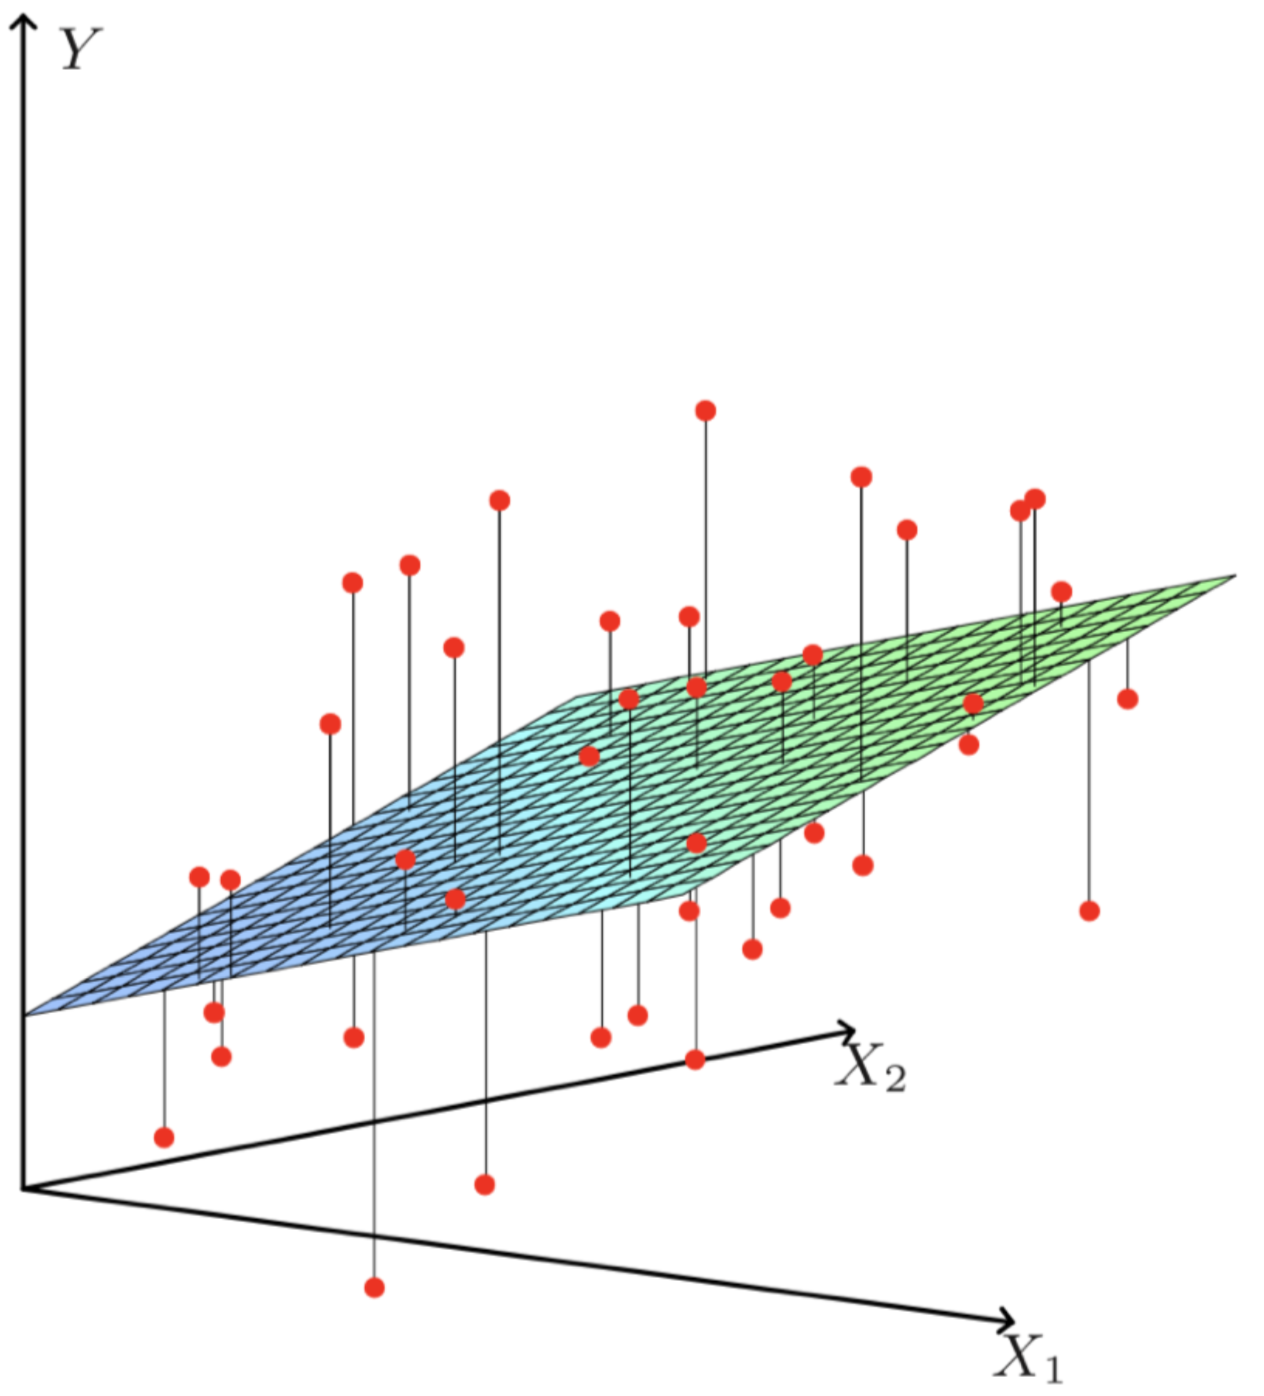
\includegraphics{./Figures/hyperplane.png}
    \caption{Linear least squares fitting with $X\in\mathbb{R}^2$. In this
        problem, we are looking for the linear function of X that minimises the
    sum of squared residuals from Y, which is an plane (hyperplane in dim 3)}
    \label{hyperplane}
\end{marginfigure}

Here, we are essentially solving a system of equations. We must consider the
number of variables adapted to the number of equations that we get. When there is
not enough equations (when $p$ is too small for example), the system is
undetermined. We cannot reduce it and do not have a single solution.

Actually, when $p>N$, we can solve this problem with the condition $\hat{l}=0$.
This is a situation where there are more parameters than there are equaltions. It
is easy to solve. The solutions consists in overfitting.

For instance if we have 100 parameters and 10 equations, we can never manage to
get any result. However, we can find easy solutions, but this will overfit.
At this stage, the system cannot be inverted.

When $p$ is large, even if it is of the same order of magnitude as $N$, we are
working with big matrixes, that can be tricky to invert with both proper
mathematical accuracy and computation performances. In such cases, we should
handle the data carefuly.

Large $p$ are typical way of using statistical learning methods, by
discriminating between datasets without having the aforesaid issues.


\chapter{General principles}
\label{ch:general-principles}

\begin{itemize}
    \item Models
    \item bias vs variance
    \item cross-validation
    \item maximum likelihood
    \item Bayes
    \item etc.
\end{itemize}


Generally, big data issues are composed of many parameters, with which it is
very energy-consuming. We usually want to reduce the problems to one or two
interesting parameters. Even if start with a lot of data, we would need to find
what are those interesting parameters, and what are the important dimensions of
the problem we will be working on.

There are two advantages at reducing the number of parameters:
\begin{itemize}
    \item[accuracy] With less parameters, we can estimate them with much more
        accuracy;
    \item[easiness] it is always easier to estimate things on a condensed set
        of parameters.
\end{itemize}

Hence the issue is to find a compromise between having enough parameters to
estimate properly the result of the problem, without loosing precision when
having a too large batch.

\marginnote{Here $||\cdot||_0$ stands for the cardinal: $||\beta||_0 = \#(\beta_j \neq 0)$}

Let $\tilde{l}(\beta)$ be defined as:
\begin{equation}
    \tilde{l}(\beta) = l(\beta) + \lambda ||\beta||_q
\end{equation}

Now, the problem lays in finding
\begin{equation}
    \min_\beta l(\beta) \; \text{given} \; ||\beta||_0 \leq C
    \; \text{with} \; \beta = [0, \ldots, \beta_i, 0, \ldots, 0]
\end{equation}

It is not possible to provide this kind of problem with any good numerical
solution. In fact, we would always try to find a compromise between what we are able to optimise efficiently and what is possible to optimise. We can
write the problem in a new version, easier to solve:

\begin{equation}
    \min_\beta l(\beta) \; \text{given}\; ||\beta||_2 \leq C_1
\end{equation}

\section{The two models}

There are two models that can be used to solve that kind of problem. The first
is the \emph{Ridge regression} that consists in using the constraints that can
be solved efficiently numerically.

The second model is called the \emph{Lasso regression} and consists in finding:

\begin{equation}
    \min_\beta l(\beta) \; \text{given} \; ||\beta||_1 \leq C_2
\end{equation}

In the ridge problem, we assume that the problem is sparse: we only need a few
parameters to capture the relationship.

In fact, the problem can be reset by writing:

\begin{equation} 
    \tilde{l}(\beta) = (Y -X\beta)^T (Y-X\beta) + \lambda \beta^T \beta
\end{equation}

\begin{eqnarray}
    \frac{\partial \tilde{l}(\beta)}{\partial \beta} &=& 2 (-X^T(Y-X\beta) + \lambda \beta)\\
    & = & 2 (-X^T Y + (X^TX + \lambda \mathds{1})\beta
\end{eqnarray}

\marginnote{$\mathds{1}$ is the identity matrix.}

We are here adding constraints to the problem, that will allow us to solve it
numerically.


\begin{equation}
C_{jk} \hfill p>N
\end{equation}
\begin{equation}
C_{jk} = \frac{1}{N} \sum_{i=1}^N x_{ij}x_{ik}
\end{equation}

\begin{equation}
\bar{x} = 0 ; C = X^TX
\end{equation}

\begin{equation}
X_{ij} \hfill  Nxp
\end{equation}

\TODO

$p>N => C$ is non invertible.\\
$N = 1, C_{jk} = x_{1j} x_{1k}$\\
$C = XX^T$ \\
here, $C$ is of rank 1.

\marginnote{remind that $Z^TZ = ||Z||^2$
\begin{equation*}
Z^T y = <Z,y> = \vec{Z}\cdot\vec{y}
\end{equation*}
}

Mathematically, $rank(C)\leq N$.

This means that there are too many parameters for too few samples. If we try to
solve this with a linear regression problem, it will give too many solutions.


Here it is easy to understand that $p>N$ cases give problems. However, because
we are working with big data, the $p\sim N$ cases also gie rise to problems. We
would need $p<< N$ to have correct solutions.

\section{Unsupervised learning}
\subsection{Example of financial data}

Let's start with stock data, as presented on figure \ref{financialdata}.

\begin{marginfigure}
    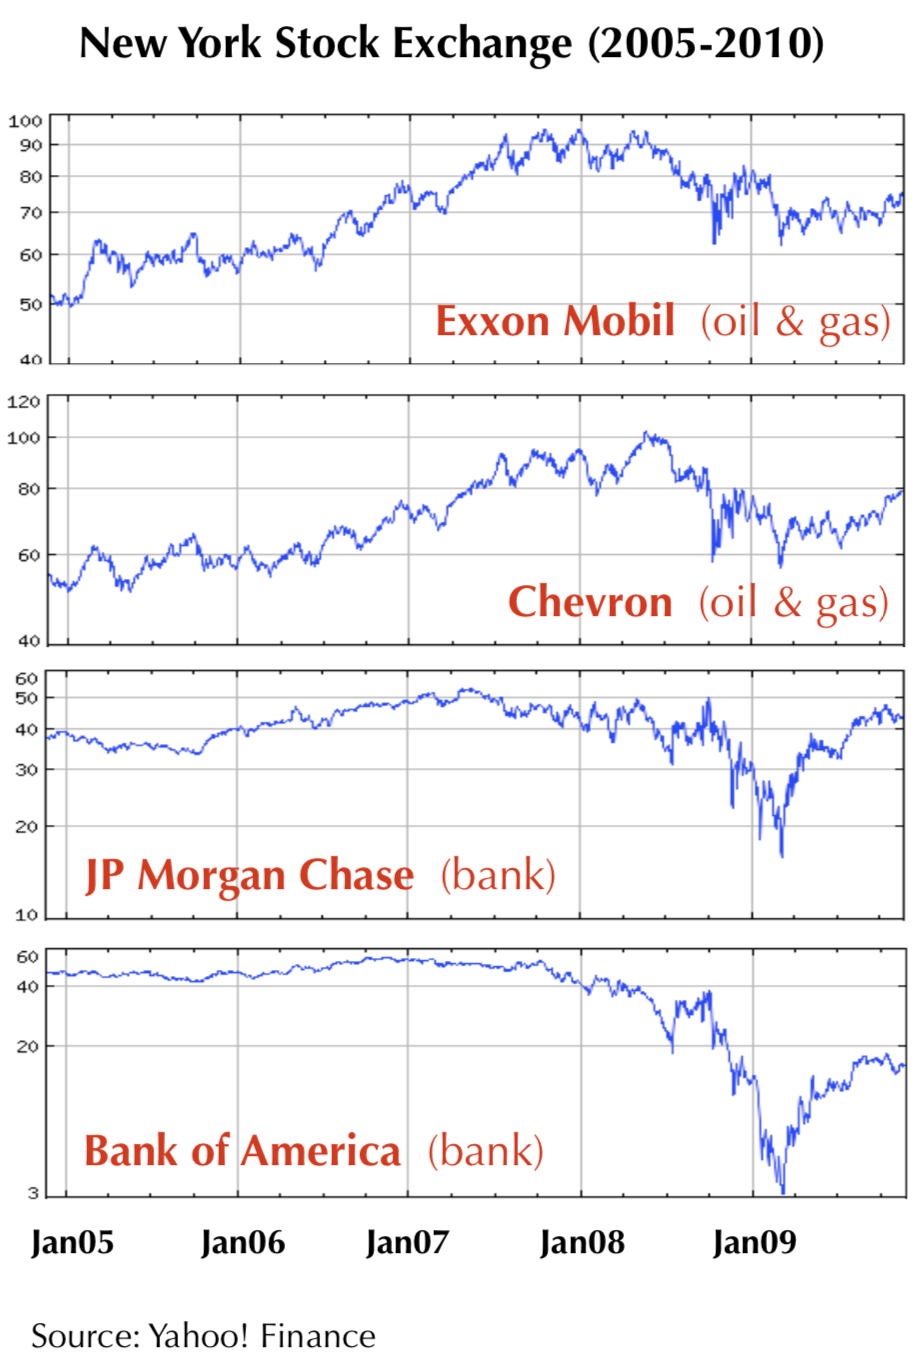
\includegraphics{./Figures/stock.png}
    \caption{Stock data used as an example}
    \label{financialdata}
\end{marginfigure}

With these data, we want to extract information. However, y data are not
labelled. For this reason, we may not use the raw data, but try to find
something else that better fits with the problem.

Let the price of stock $i$ at time $t$ be $s_i(t)$. The stock index i can vary
from 1 to $p=1,000$, and the data are separated with a time interval 
$\Delta t = \SI{30}{\minute}$. The time variable $t$ ranges from 1 to $N=6228$
(that represents 2 years).

Let us define the following variables:

\begin{eqnarray}
    r_{ti} & = &  \ln \frac{s_i(t+\Delta t)}{s_i(t)}\\
    x_{ti} & = & \frac{r_{ti} - \bar{r}_i}{\sigma(r_i)}\\
    C_{ij} & = & \nth \sumin x_{ti} x_{tj} 
\end{eqnarray}

Here, we want to get rid of the $\alpha$ parameter; for this reason, we use the
$r_{ti}$ data instead of the $s_i(t)$ parameter.

Then we define $x_{ti}$, by substracting the mean and normalising with the
standard deviation.

Therefore, the $x_{ti}$ value has a null mean, and a standard deviation rescaled
to 1. Hence we have rescaled the problem so that each data vary within the same
range.

Now, let's move to the data $C_{ij}$ that represents the correlation between two
$x_{ti}$ variables. The matrix $C$ of $C_{ij}$ coefficients is of great interest
in our problem.

\marginnote{NB: When we consider some data, it is usually very important to
    watch it before trying to compute anything else. Particularly, if something
    looks obvious to the eye, we need to set it clearly, before trying to
    interpret it with the math.
}

Before trying to make anycalculation, we can assume that Exxon's and Chevron's
data are strongly correlated, as well as JP Morgan's and Bank of America's.

Thus, we may suppose that $C_{Ex,Ch} > C_{Ex,JP}$.

In order to analyse the data, we may compute the spectrum. 
Or see clearly from the definition that the matrix is symmetric, and has all the
properties to be diagonalised.

\begin{equation}
    C_{jk}, C_{jj} = 1 ; C_{ij} = C_{ji}
\end{equation}

Thus we get the eigenvalues: $\lambda_1, … , \lambda_p$, and the eigenvectors
$v_1, … , v_p$. The dispersion of the eigenvalues is represented on figure
\ref{fig2}.

\begin{marginfigure}
    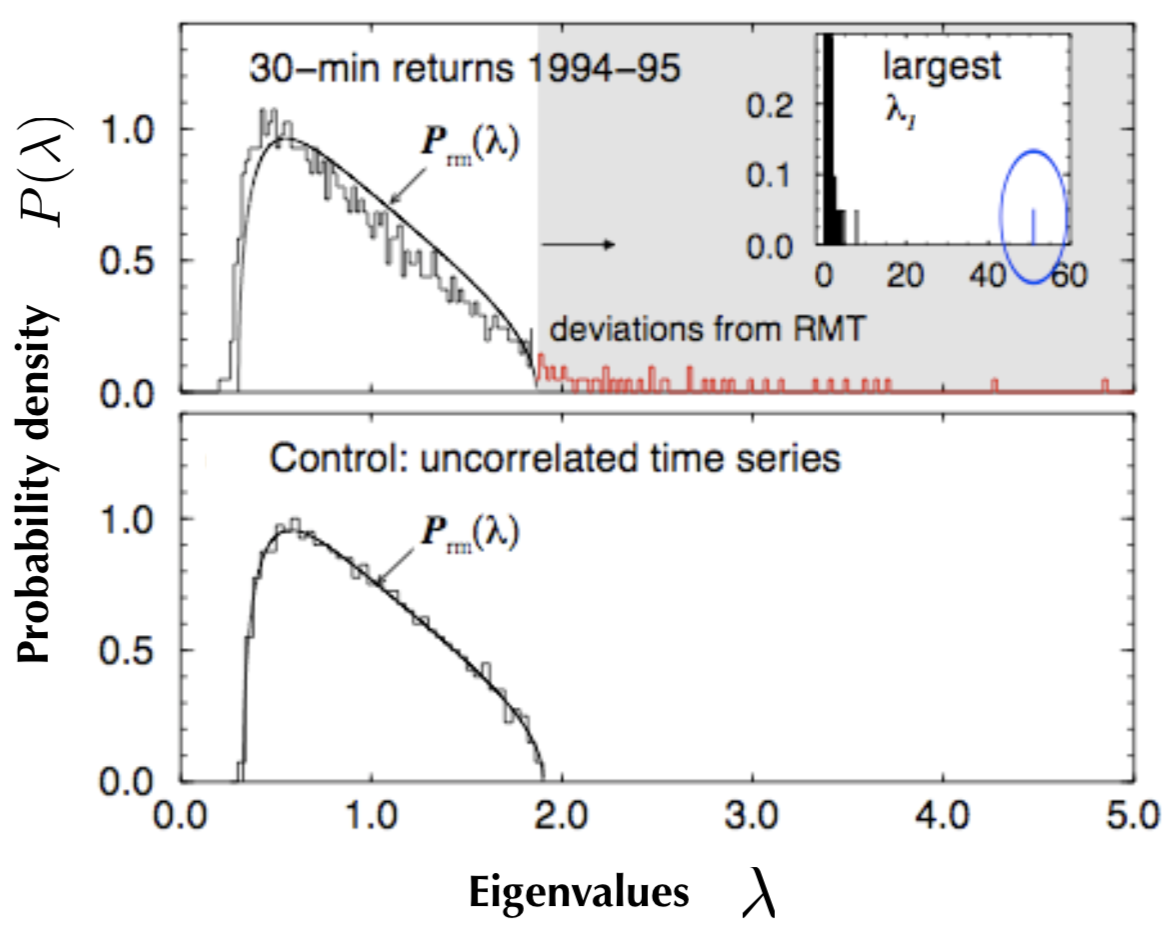
\includegraphics{./Figures/eigenvaluesdisp.png}
    \caption{dispersion of the eigenvalues}
    \label{fig2}
\end{marginfigure}

The bottom part of the graph presented on figure \ref{fig2} is called the
control part. Actually, we see that this part comprises mostly noise, and the
interesting part of the data is the upper part, that describes longer range
correlations.

The control part just shuffles the data, and is due to permutation of the values
. If we randomly shuffle the data, to remove all the interesting information
(correlation between the different stocks), the control part stays the same.
This is actually a way to see what kind of correlation we can get from just
randomness, in a case where there is no correlation from the data.
Thus, we can quantify the degree of noise. Because 98\% of the eigenvalues are
contained in the 1st part of the data (control), it means that the stock data
are comprised of 98\% of noise.

Let's write the matrix C as:
\begin{equation}
    C = \sum_{j=1}^p \lambda_j v_j v_j^T
\end{equation} 
\begin{equation}
    v_j^T v_k = \delta_j^k
\end{equation}

With the random metrics theory (RMT - branch of statistical physics), it is
possible to compute analytically the shape of the control series:

\begin{equation}
    \min_x l(x) \; \text{given} \; g(x)\leq C
\end{equation}
\begin{equation}
    \min_x l(x) + \lambda g(x) \; \text{with} \; \lambda \geq 0
\end{equation}

\begin{marginfigure}
    \TODO
    \caption{scheme}
    \label{fig3}
\end{marginfigure}

We assume that everything is differentiable, therefore:

\begin{equation}
    \nabla_x l(x) = -\lambda \nabla_x g(x)
\end{equation}

The conditions impose that the two gradients should be aligned, and directed
in opposite directions. More generally, it would depend on the value C.
There is a minimum value, but if the problem is not perfectly shaped, the
minimum we would get can be a local minimum instead of an absolute minimum. This
threatens the issue resolution.

Let's suppose we have $l(\beta)$. We may now consider the norm of $\beta$ to be
lower than the C value:
\begin{equation}
    ||\beta||_q \leq C_q
\end{equation}

Of course, this can also be done with different norms, like $l_0$, $l_2$,
and sometimes also with the $l_1$ norm.

\subsection{Example: crime data}

Let's give a few examples related to such a problem. We start with the data
presented in figure \ref{crime}

\begin{figure}
    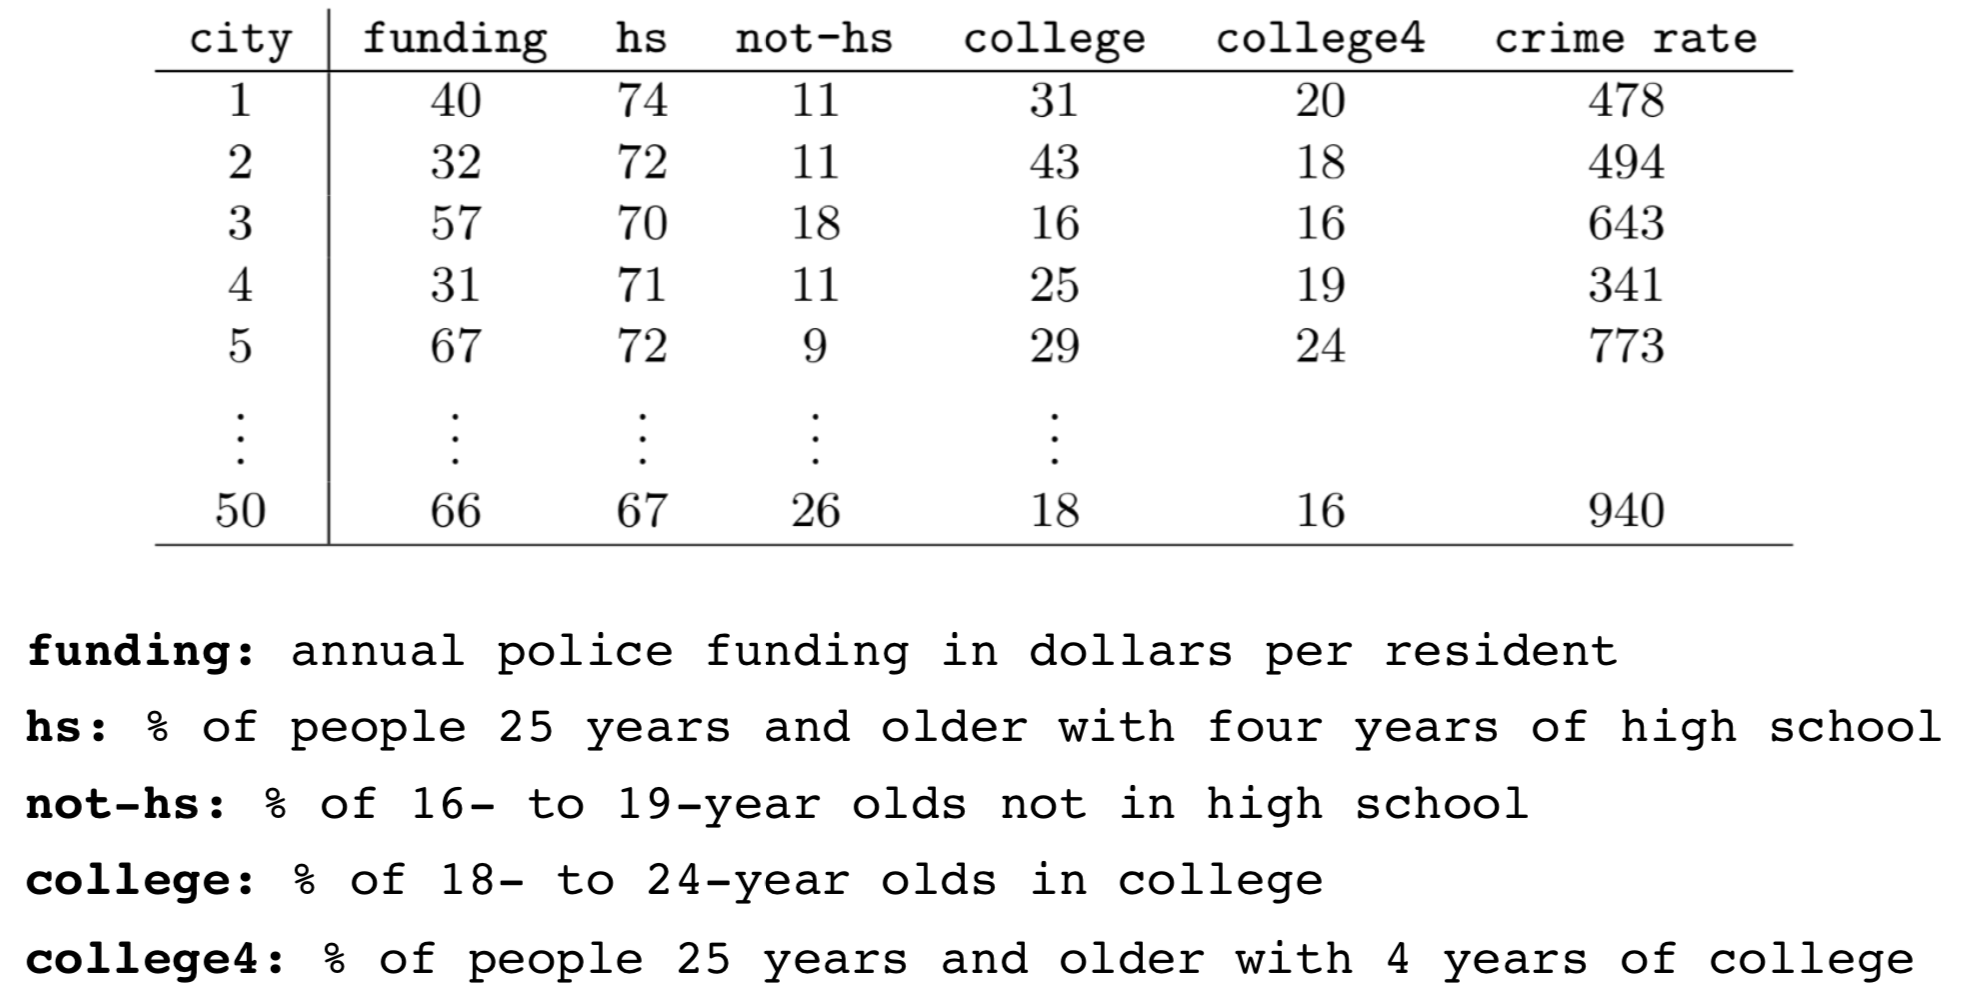
\includegraphics{./Figures/crime.png}
    \caption{Example: crime data, crime rate and five predictors for $N=50$ U.S.
    cities}
    \label{crime}
\end{figure}

These are not too big data: $N=50$ and $p=5$.
With a not too big dataset, taken from a book. The goal here is to try to
predict the crime rate, and to what it is correlated.

$(x_{ij}, y_i)$ $i=1..N=50$ cities
$j=1…5$

The idea is to consider naively a simple problem.

Here we may find linear combination of all different problems.
For a physicist, it seems we’re not allowed to to so, because it is not
homogeneous. However, this helps in finding correlations.

\begin{equation}
    x’_{ij} = x_{ij} - \bar{x_j}
\end{equation}

In this case, we have zero mean, We may also want try to divide by the standard
deviation. This is not the case here.

\begin{equation}
    y=\sum_{j=1}^p \beta_j x_j
\end{equation}

Therefore we can write the relation:

\begin{equation}
    l(\beta) = \frac{1}{N} \sum_{i=1}^N (y_i - \sum_{j=1}^p \beta_j x_{ij})^2
\end{equation}

The result of this optimismation may be given as a function.

Let's represent the results for the Ridge regression on figure \ref{ridgecrime}

\begin{marginfigure}
    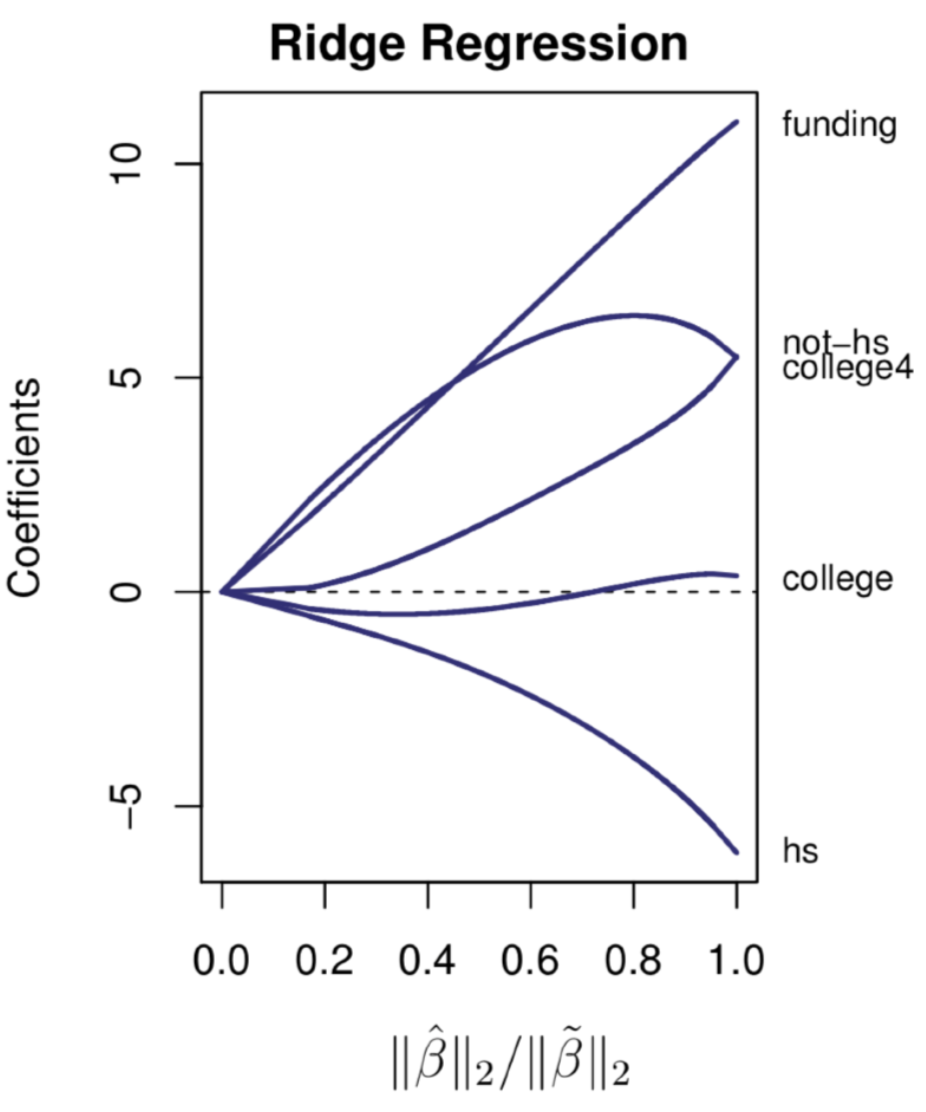
\includegraphics{./Figures/ridgecrime.png}
    \caption{Coefficient path for the ridge regression, plotted versus the
        relative $l_2$ norm of the coefficient vector, relative to the norm of
        the unrestricted least-square estimate $\tilde \beta$
    }
    \label{ridgecrime}
\end{marginfigure}


What is plotted is the value of the $\beta$ along the $x$ axis. This is related
with the cost ($c_q$). 
We can repeat for different values of the cost.
If we do it for large $C$, we do not put any constraints, and therefore get the same $\beta$.

If we put a very strong cost, like $0$, the only solution is $\beta = 0$.
Hence we’re looking at different solutions, constrained, and then we relax it to
a state where there’s no constraint anymore.

Now, let's represent the results for the Lasso regression, on figure
\ref{lassocrime}.
\begin{marginfigure}
    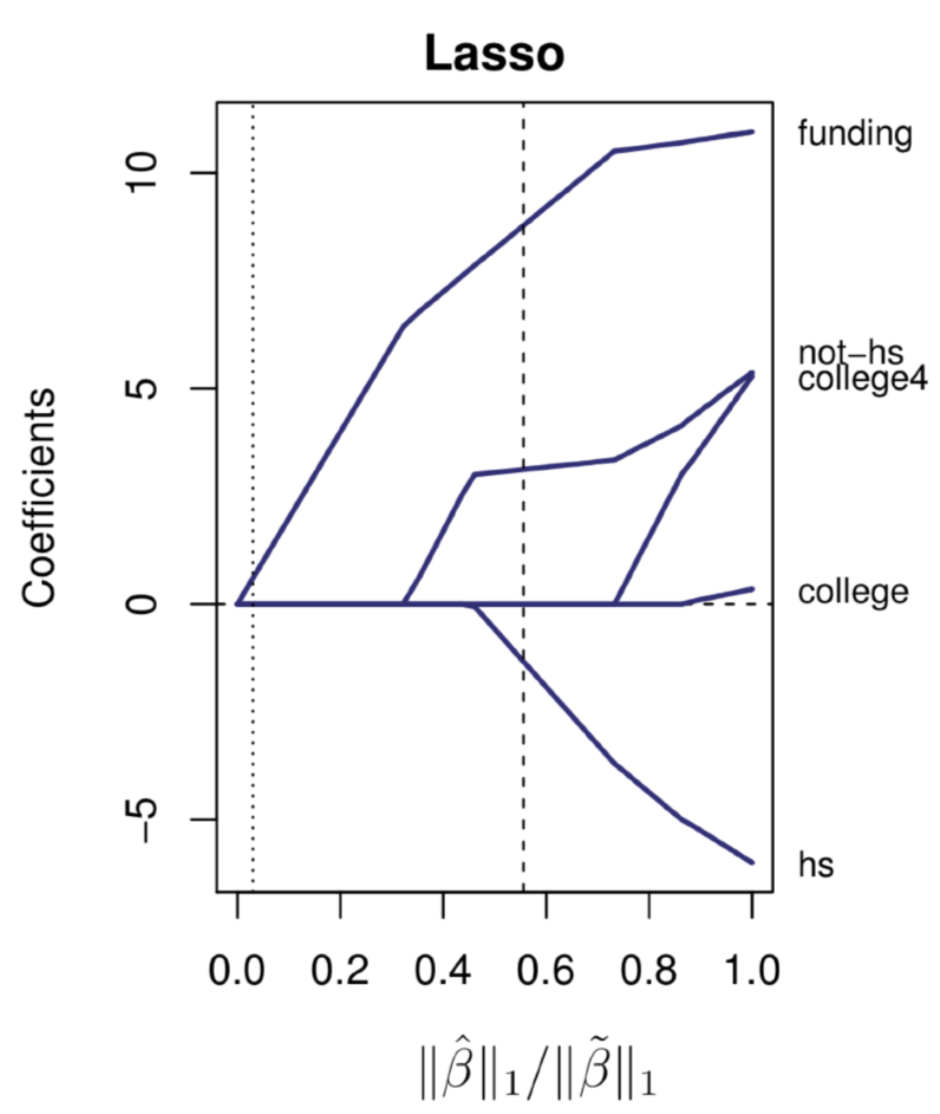
\includegraphics{./Figures/lassocrime.png}
    \caption{Coefficient path for the lasso regression, plotted against the
        relative $l_1$ norm of the coefficient vector, relative to the norm of
        the unrestricted least-square estimate $\tilde \beta$
    }
    \label{lassocrime}
\end{marginfigure}

The lasso graph is the same, but performed with $l_1$ norm.

There’s a way to understand this, by giving an illustration of the sparsity from
$l_1$ constraint, as shown on figure \ref{sparsity}.

\begin{figure}
    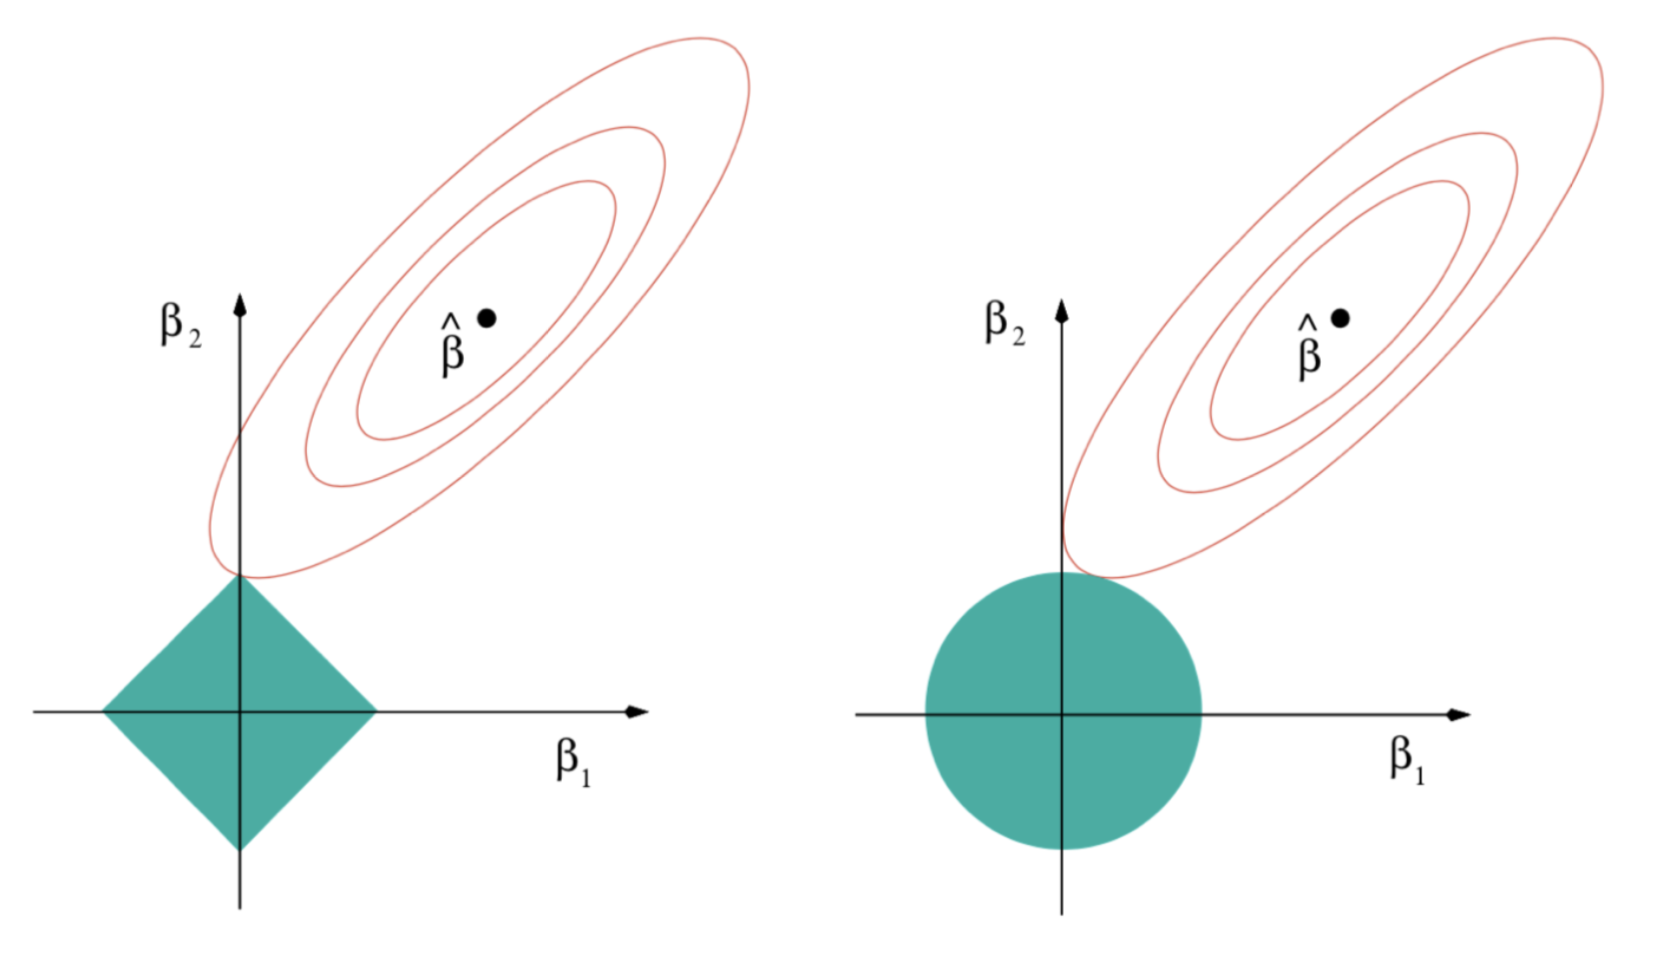
\includegraphics{./Figures/sparsity.png}
    \caption{Estimation picture for the lasso (left) and the ridge regression
        (right). The solud blue areas are the constraint regions
        $|\beta_1| + |\beta_2| \leq t$ and $\beta_1^2 + \beta_2^2 \leq t^2$,
        respectively, while the red ellipses are the contours of the residual-
        sum-of-squares function. The point $\hat \beta$ depicts the usual
        (unconstrained) least-squares estimate.
    }
    \label{sparsity}
\end{figure}

\TODO: introduction à cette équation.
\begin{equation}
    y=F(x,\theta).
\end{equation}

Linear models yield to:
\begin{equation}
    F(x,\theta) = \sum_{j=1}^p \theta_j x_j
\end{equation}

The principle hire is to have the results of $p$ data, and then, once we get 
another dataset -- similar to the previous one -- we will be able to fit it and
to find the solution:
\begin{equation}
    x_1, \cdots x_p, x_1^2, \cdots, x_p^2, \cdots cos x_1, \cdots
\end{equation}

\begin{equation}
    F(x, \theta) = \sum \theta_j h_j(x)
\end{equation}

Later on, we will introduce neural networks. In this case, the function people
are more familiar with will be:

\begin{equation}
    h_j(x) = \frac{1}{1 + \exp (-\omega_j^T x )}
\end{equation}

Where $\omega_j$ is the weight that adjusts the coefficients.

Here, it becomes clear that there is a relation between $x$ and $y$. Considering
this, there is now no limit to the complexity of the problem we can take.

At this stage it becomes necessary to define a loss function $L$. This can be
written as in equation \ref{lossfunc}.

\begin{equation}
    L (y, F(x, \theta)) = (y-F(x,\theta))^2
    \label{lossfunc}
\end{equation}

With any given model and loss function, we need to define a training error
$\varepsilon_{train}$, as shown in equation \ref{trainerr}.
\begin{equation}
    \varepsilon_{train} = \nth \sumin L (y_i, F(x_i,\theta))
    \label{trainerr}
\end{equation}

The training error is of utter importance. However, this will not be the only
quantity we will have to consider.
In fact, there is also a test/generalisation error. This one would be the error
we get when we are using these datapoint that have not been used in the training
of the problem.

There’s the training set, used to learn the parameters, and the additional data,
on which we’re going to apply the model, and to try to generalise the data that
have been used as an input for the fit.

\begin{marginfigure}
    \includegraphics{./Figures/traintesterror.png}
    \caption{Training vs test errors}
    \label{traintesterrors}
\end{marginfigure}

\begin{equation}
    \varepsilon_{test} = \frac{1}{N’} \sum_{i=1}^{N’} L(y_i’,F(x_i’,\theta))
\end{equation}

Let's plot the training error $\varepsilon_{train}$ in comparison with the test
error $\varepsilon_{test}$ on figure \ref{traintesterrors}. The test errors have
been traced in red while the training errors have been traced in blue.

\section{k-fold cross validation}

Our objective here is not to get the best fit, but to generalise the given data.

The procedure we will chose is called \emph{k-fold cross validation}. It
consists in dividing the data in 5 datasets and then take one out of these to
be used a the test, and all the others as the training sets.
This is then repeated for all the other combinations. The data are divided in
$K=5$ or $10$ and then most of the data are used to train the algorithm, while
the last set of data is used to test the algorithm.

In this procedure, the data set is splitted in:
\begin{itemize}
    \item training set (for the fit) (\eg 50\% of the data)
    \item test set (for model selection) (\eg 25\% of the data)
    \item validation set (for assessment) (\eg 25\% of the data)
\end{itemize}

This is used to better understand how to find the best parameters leading to the
best fit.

Let's take our previous example:
\begin{equation}
    y=F(x)
\end{equation}

The training set may be described as: $\hat{\theta}$

The model is $y=F(x,\theta)$

Thus we have $y= \hat{F}(x) = F(x,\theta)$.

Now, let's work with another dataset:

$x_0$
\begin{equation}
    \E [(F(x_0) - \hat{F}(x_0) )^2]
\end{equation}
 
Here, $\hat F$ is the prediction.

This is considered over different training sets. It says how far we are from the
value we want to predict.

\begin{equation}
    \E[(F(x_0) - \hat{F}(x_0) )^2] = F(x_0)^2 - 2F(x_0) \E (\hat{F}(x_0)) + \E (\hat{F}(x_0)^2)
\end{equation}

Where $\E (\hat{F}(x_0)^2)$ is $\var(\hat{F}(x_0) + (\E[\hat{F}(x_0)])^2$

\ie $\E[(F(x_0) - \hat{F}(x_0) )^2] = (F(x_0) - \E[\hat{F}(x_0)]^2 + \var(\hat{F}(x_0))$.

The test error may be written as the sum of the variance and the square of 
the bias.

\begin{equation}
    \varepsilon_{test} = bias^2 + \var
\end{equation}


This can be generalised with the addition of a random variable $\epsilon$
designating some noise:

\begin{equation}
    y = F(x) + \epsilon
\end{equation} 

Here it becomes necessary to add the irreducible error $\var(y)$

In the context of linear regression, one may apply the Gauss-Markov theorem.
This one tells us that in linear regression, when considering all the estimators
that have no bias, the best one is the one that minimises the loss function
presented in equation \ref{lossfunction}. 
\begin{equation}
    L(y,F(x)) = (y-F(x))^2
    \label{lossfunction}
\end{equation}
This theorem shows that if one is interested in minimising the bias, in the
context of linear regression, he should consider $\min_\beta l(\beta)$

The absence of bias and the minimum variance is obtained for
\begin{equation}
    \min_\beta l(\beta)
\end{equation}

In general, the best solution is not the solution that has no bias.
Hovewer, a better estimation of the parameters can be found when the set of data
will be constrained.

\section{bias VS variance}

\TODO

%last time, we learnt unsupervised learning.
%$(x,y)_{i=1\cdots N}$

%Goal : learn $x \rightarrow y$. function: theta
%so that when given new $x_i$

%$x_i \rightarrow^{predict} \hat{y_i} \sim y_i$
%function: $\hat\theta$


%function with two components : $err_{test}$ wich is composed of the bias +
%variance.
%if large amount of data, high variance, very hard to learn, and we get
%very different parameters.

%we may want to compromise this with a model with less parameters with 
%a lower variance problem.
%not only we want to pick the best variable in the model, but also the model
%itself.
%we consider a class of problems, described with a parameter $\lambda$.
%we introduce $\lambda$ as a parameter of regularisation.

%\marginnote{we are defining, for example, the error as:
%\begin{equation*}
%    l(\beta,\lambda) = \frac{1}{N}\sum_{i=1}^N (y_i - \beta x_i)^2 - \lambda ||\beta||_0
%\end{equation*}
%}

%\begin{itemize}
%\item training -> $\hat \theta$ given $\lambda$
%\item validation -> $\hat \lambda$
%\item test -> $Err_{test}$
%\end{itemize}

%At the begining, we divide the dataset into multiple datasetts.

%K-fold cross validation : the idea is that we have one dataset, that we divide
%into K subsets. We can get it with statistics. two weeks ago, we've seen an example of this, in the context of linear regression.
%minimising the mean square error

%planning of the day:
%\begin{itemize}
%\item Bayesian approach
%\item how we do the approximation in practice.
%\item example of CLASSIFICATION.
%\end{itemize}

\section{Maximum likelihood}
Let's discuss about the maximum likelihood estimation (MLE). We must keep in
mind that this a general approach in statistics and not a big-data specific one.
In general, we would consider a model of the form $y= f(x,\theta)+ \epsilon$,
where $\epsilon$ is a random variable that stands for the noise.

We may assume at a first sight that $\epsilon$ is a normal variable:

\begin{equation}
    \epsilon \~ N(0,\sigma^2)
\end{equation}

The probability to get $x$ with $\theta$ may be written as:
\begin{equation}
    P(y|x,\theta) = \frac{1}{\sqrt{2\pi\sigma^2}} \exp - \frac{(y-f(x,\theta))^2}{2\sigma^2}
\end{equation}

\begin{marginfigure}
    \TODO
    \caption{$P(y|x,\theta)$ representation. with the standard deviation $\sigma^2$ and centered on $f(x,\theta)$}
    \label{gauss}
\end{marginfigure}

Now, let's imagine we are given a set of values $(x_i,y_i)$. We want to find
the best parameter $\hat \theta$. For this, we can look at the parameter that
make the data the most likeable.

\begin{eqnarray*}
\mathcal{L} (\theta|Z_1,\cdots,Z_n) & = &  \log P(Z^N|\theta)\\
    & = & \sum_{i=1}^N \log P(Z_i|\theta)\\
    & = & \sum_{i=1}^N \left[ -\half \log (2\pi\sigma^2) - \frac{1}{2\sigma^2} (y_i - f(x_i,\theta))^2 \right]\\
    & = & - \frac{N}{2} \log(2\pi\sigma^2) - \frac{1}{2\sigma^2} \sum_{i=1}{N} (y_i -f(x_i,\theta))^2 \\
    &=& -\frac{N}{2} \log(2\pi\sigma^2) - \frac{1}{2\sigma^2} l(\theta)
\end{eqnarray*}

All we have considered until now is just a mean squared deviation (MSE) approach
. The MLE approach can be written as:

\begin{equation}
    \max_\theta \mathcal{L}(\theta,Z^N) \rightarrow \hat\theta
\end{equation}

Thus we may get the following theorem:

if $y$ can be written as the sum of $f$ and a random variable bias $\epsilon$: 
$y =f(x,\theta_0) + \epsilon$, then the expected value $\E$ tends towards
$\theta_0$ when $N$ is sufficiently high.
\begin{equation}
    \E[\hat\theta] \xrightarrow[N\rightarrow\infty]{} \theta_0
\end{equation}

Where $\hat\theta \~ N(\theta_0, F(\theta_0)^{-1})$

$F(\theta) = \E\mathcal{L}(\theta)$ this is called the Fisher information.

$I(\theta)_{ij} = - \frac{\partial^2 \mathcal{L}}{\partial \theta_j \partial\theta_k}$

Therefore,

$\hat\theta \sim (approx) N(\hat\theta, I(\hat\theta)^{-1})$

\begin{marginfigure}
\TODO
figure parabolle inversée, maximum : courbature $-\partial\mathcal L/\partial \theta^2$, absisse max : $\theta_0$. ordonnée : L.
\end{marginfigure}

We want to find the best parameter, \ie the one that is the more likelihood to be \ldots

$\mathcal{L}$ is called the log-likelihood. P is colled the likelihood.
In a sense, we want to find the most likely model.

We can mention, that there are two difficulties :
\begin{itemize}
\item we need to find the maximum
\item problem of validation: if we have a more complicated model, we would increase the log likelihood, and no way to do the validation.
\end{itemize}

\section{Bayesian approach}

Now, another approach: the Bayesian approach. Again, this is not specific to big-data.
We may know that there are lot of debates in the meaning of probabilities. There
are two schools: the frequentists: probabilities have a meaning only when the
event is reapeating many times. Like a coin tail or head. Fundamentally, if I do
it a large number of time, this is converging.
If we take an event that can happen only once: the probability that there's lifeon the moon: for a frequentist, there's no meaning.
the Bayesian view is different in nature: probability is not about counting, but
about biliefs. This represent how I believe the event to be actually the case.
Concretely, the idea of the bayesian approach is:
elementary probability: when I have two random variables X, Y.
The joint probability of (X,Y): P(X,Y). we can also define the marginals :
$P(X)$, $P(Y)$, that are only the probability $P(X) = \sum_y P(X,Y)$.
$P(X|Y)$: conditional probability.
$P(X,Y) = P(X|Y)P(Y)$
therefore $P(X|Y) = \frac{P(X,Y)}{P(Y)}$.


$P(Z,\theta) = \frac{P(Z,\theta)}{P(Z)} = \frac{P(Z|\theta)P(\theta)}{P(Z)}$.
This is called the Bayes formula.

$P(Z=1) = \theta$
$P(Z=0) = 1-\theta$, for example, for a binomial problem.

$P(Z|\theta)$ is the likelihood I had before.
In this approach, there's something new, that is $P(\theta)$ wich is called the prior.
For a bayesian, we always have some \emph{a priori} bieliefs about the
distribution of the parameters. When I see the data, I have to update my
beliefs.
$P(\theta|Z)$ is called the posterior.
$P(Z)$ is called the evidence.

Here we have to do the inference, that is the general model. Usually, when we
look at probabilites, we look at $P(Z|\theta)$. reverse approach.
We look at  the model, that also incorporates the prior.

On the slides, one partialicular example of the prior to solve a praticular problem.

\section{In practice\dots}
Here, there's nothing to do with big data. example taken from the book of MacKay
example: Jo has a test for a disease. a = state of health.
a=1 if sick, 0 otherwise.
the test is giving another variable b
what is known about this test is that it can be positive even if there's no
disease. $P(b=1|a=1) = 95\%$. same for zero.
it means the test gives the right result in 95\% of the cases.
we need to know the case when somebody of HIS AGE has the disease. this
is gonna be the prior. $P(a=1) = 1\%$.
The exercise is to find what is the probability $P(a=1|b=1)$.
In the bayesian approach, we do not have a theta, but a distribution of the theta
we always have a probability to have different values, especially the maximum
\emph{a posteriori} estimate (MAP)
which is given by taking the max of this:
$\max_\theta P(\theta|Z)$.

It will give the same results if we are assuming that this is not depending on theta. If we have a flat prior.
Then, this is equivalent to the MLE.

When I'm maximising the posterior, it means I'm maximising the likelihood.
Thus we can see the likelihood as a bayesian approach, with a partialicular prior
value.

Let's say we have the same model as before. This time, we assume the prior is
a one dimensional variable, with a gaussian distribution.

$f(\theta)  = \sqrt{\frac{\lambda}{2\pi}} e^{-\lambda \frac{\theta^2}{2}}$

Then, this will be very similar to the l validation, if we take the log of this.
Then, this is multiplied by lambda theta square over two.

When we take a prior on these parameters, we want to give more probability to
the small values of the parameters. width of the gaussian: 1/sqrt(lambda).
control the probability of the parameter to have a large value.
restricting the range of the parameter that we are considering, as we saw before

The goal here is to present this partialicular approach, and recover the maximum
likelihood.
An interesting aspect of the bayesian approach. Again, this is very general.
Let's say that, in general, we have the probability of the data, given some
hypotheses:

$P(D|H_1)$
Dis the data, $H_1$ thehypothesis.

we want to compare with another hypothesis: $P(D|H_2)$

What the bayesian approach is telling us is that we have to consider the
probability :
$\frac{P(H_1|D)}{P(H_2|D)} = \frac{P(D|H_1)P(H_1)}{P(D|H_2)P(H_2)}$

it depends on the prior we put there. we do not here have no belief????

One example of the maximum likelihood and the general approach.

Problem of generalization.
Let's say we have the data:
$x_{i=1\ldots N}$. two approaches are possible:
MLE that gives $\hat\theta$
bayesian that gives $P(\theta|X)$.

what is the probability of a partialicular value?

$P(x_{N+1}) = $(MLE) $P(x_{N+1}|\hat\theta)$. if we need a best value of approximation, let's replace the parameter.

= (bayesian)$ P(x_{N+1} | X^N) = \sum_\theta P(x_{N+1}|\theta P(\theta |x^N)$

here, $P(\theta |x^N)$ should be used as the new prior. We are constantely updating our believes. this is the prior we get before knowing the
value,
depending on what we saw before. This has to be equal to:
$\frac{P(x^N|\theta)P(\theta)}{P(x^N)}$

There's a famous problem that has to do with that: the rule of succession.
The sun is rising every morning, what is the probability it will rise tomorrow?
Laplace discussed this issue.

With different approaches, we may get different results. One of the simplest
example.
Let's assume there's some probability $\theta$ the sun is rising in the morning.
We hae a binomial model. This is the same issue as a coin that always ends up
in the same edge: tail for example.
Maximum likelihood estimation: the probability would be 1.

$x_i = 0/1.$

$x^N = (x_1, \ldots ,x_N) = (1,\ldots,1)$

$P(x_{N+1} = 1) = ?$
If we do the maximum likelihood approximation, this would be 1 everytime.

$X^N : N_1 times 1 ; N-N_1 times 0.$ (times : frequency it happens over time)

$P(x_i|theta) = \theta$. One parameter model, binomial model.
Obviously, the probability $P(x_i=0|\theta) = 1 - \theta$. this example cannot be
simpler than this.


theta can be anything between 0 and 1. $0 \leq \theta \leq 1$.

I'm giving the same probability for every $\theta$. $P(\theta) \sim $uniform.

$P(x_{N+1} =1|x^N) = \int d\theta P(x_{N+1}=1|\theta) P(\theta|x^N)$
$= \int d\theta \theta \frac{P(x^N|theta)P(\theta)}{P(x^N)} where P(\theta) = 1$
$= \frac{N!}{N_1!(N-N_1)!} \theta^{N_1} (1-\theta)^{N-N_1}$

The difficulty lies in the $P(x^N)$ that does not depend on theta.

$P(\theta|x^N)=C(N,N_1) \theta^{N_1} (1-\theta)^{N-N_1}$

$\int d\theta P(\theta|x^N) = 1$

$\int_0^1 d\theta \theta^a (1-\theta)^b = \frac{a!b!}{(a+b+1)!}$
this exists also for a and b that are not integer values, and this is called the
gamma function.
If we use this formula, we would find this to be:

$c(N,N_1) = \frac{(N+1)!}{N_1!(N-N_1)!}$
with the proper normalisation.
I need just one line to compute the stuff.
If I compute this:

$P(x_{N+1}=1|x^N) = \int_0^1 d\theta \theta \frac{(N+1)!}{N_1!(N-N_1)!} \theta^{N_1} (1 - \theta)^{N-N_1}
= \frac{(N+1)!}{N_1!(N-N_1)!} \frac{(N_1 + 1)! (N-N_1)!}{(N+2)!}
= \frac{N_1 + 1}{N+2} \neq \frac{N_1}{N} (MLE)$

this is called as the laplacian formula.

we have a non-zero probability to observe something that we have never observed
before.

$N=3. X^N = (1,1,1). can we bet that x_4 = 1?$
maybe it is not very wise to say this. this rule takes this into account. here, the probability to be 0 will be 1/5, not zero.

people that carry out statistics use pseudo-counts. we are adding one zero and one one.
It is a way to regularise the variation.
In this case, a frequentist would say that we have too few points and that we
must give up the problem. for a bayesian, the calculation would be very
dependant on the prior.
Prediction on the next outcomes.

commentary:
$I(\theta) = -\frac{\partial^2 \mathcal{L}}{\partial \theta_i \partial \theta_j}$

$\mathcal{F} (\theta) = \E [I(\theta)]$
MLE: $\hat\theta \~N(\ldots)$
For each dataset, we can use another expectation. It is mathematical consideration,
considering all the possibilities of my data.If we arepartialificially generating
data 
when we want to prove all mathematical results analytically, we need all the
possible datasets that we can get.
variance about everything we can get when generating different datasets.







second hour.



Now I want to discuss the computational issues.

$\hat \theta$ that I want to maximise. 
log likelihood: $\mathcal{L}(\theta|x^N)$. we would have, in general, to get these
data numerically, and not analytically, with optimised function. compromises to
be done.

Very simple, but the problem can be complicated if the function has several minimum.
Let's assume the problem is convex: the function is convex, as well as the set
of data.
Any global minimum is a global minimum. It can be generate, but,\ldots

In all these problems, we can consider a gradient descent.

If we want to minimise the function,

scheme fig 2.
If we look at the gradient, and spartial from a point (random). we look at the
grandient, and move in the direction of it.
we usually take a very small displacement. spartial iteratively.

$\theta_{t+1} = \theta_{t} - \eta \left( \frac{\partial L}{\partial \theta}\right)_{\theta_{t}}$

scheme: cf notes.

cf learning rate, etc.

$L(\theta) = \sum_{i=1}^N (y_i - f(x_i,\theta))^2
= \sum L_i(\theta)$.
for each calculation, we have to recompute the data.
a version of this algorithm is used very often, and is called stochastic gradient.
What we do is: compute $L_i(\theta)$ for a subset of the points.
So we take a subset of samples to estimate $L(\theta) = \sum_{i\in subset}$ and we
change at each iteration.
The sample is called mini-batch.

There's one version of this algorithm, where everytime we take a single value as
a subset: subset =1. this is called on-line learning. in this case, what we are
doing is:

$\theta_{t+1} = \theta_{t} - \eta \nabla_\theta L_i(\theta_{t})$.

The issue is to get faster. In general, we have to take the sum.
At the end, it is equivalent to do a move at everytime than getting the sum from
the very beginning.
Actually ,this algorithm is very powerful. In neural networks, backpropagation
is nothing more than this algorithm put in application.

This is really a local method. If I spartial from one point, I can end somewhere
different. I can be trapped in local minima. It is really difficult to find the 
correct minimum. That's why we usually work with convex functions, where local
minima do not exist elswhere than the global minimum.

$l_0$ norm, $l_1$ norm.
$||\beta||_0 = \# nonzero \beta_j ; ||\beta||_1 = \sum_j |\beta|_j$

For this reason the closest problem to the first is with $l_1$, and it is convex
so that it can be solved with an iterative method. Generally, these are
considerations we want to take into account.
We will see examples of doing this next time.

Next week: exercise as homework. practical.
that will be the grade.

$min_\beta L(\beta) -> \hat \beta$

Lasso regression.
this is one in which we are going to impose a condition:
$||\beta|| \leq t$
this is equivalent to the fact that we want to minimize :
$min_\beta L(\beta) + \lambda ||\beta|| with some parameter \lambda.$

ridge regression: $||\beta|| = ||\beta||_2^2
= \sum \beta_i^2$

if we take the $l_1$ norm:

lasso regression: $||\beta|| = ||beta||_1 = \sum |\beta_i|$

At this stage, we can take it as an exercise.

Le'ts spartial with the function I want to minimize.
$\mathcal{L} (\beta) = \frac{1}{N} \sum_{i=1}^N (y_i - \beta x_i)^2 + \lambda |\beta|$

differentiation: we must be careful.

$\frac{\partial\mathcal{L}}{\partial\beta} = 0$

the maximum, if $\beta$ is positive ,let's say, we can get the value:
$(\beta >0)$

$\frac{\partial\mathcal{L}}{\partial\beta} = - \frac{2}{N} \sum_{i=1}^N (y_i - \beta x_i)x_i + \lambda.$

I would take $\bar{x} =0, \bar{y} = 0$ and $\overline{x^2} = 1$. normalise all the
data.

In general, everything can have completely different units. It makes sense here
to normalise, so that each data has the same range of variation.
So

$dL/d beta = -2 (\frac{X^T y}{N} - \beta) + \lambda = 0$

thus $\hat \beta = \frac{X^Ty}{N}- \frac{\lambda}{2}$

If $\frac{X^Ty}{N} > \frac{\lambda}{2}$, thus
$\hat{\beta} = \frac{X^Ty}{N} - \frac{\lambda}{2} >0$

if $\beta < 0$, then we can use the same approach.

$\hat \beta= S_{\lambda/2} \left( \frac{X^T y}{N} \right)$

$S_a (u) = \sign(u) \max(O,|u|-a)$. soft-thresholding operator. cf figure notes.

This is a figure for p=1.

cf on the website a slide with the formulas.

for $p>1$,

$L(\beta) = \frac{1}{N} \sum_i (y_i - \sum_k \beta_k x_{ik} )^2 + \lambda \sum_k |\beta_k|$

$= \frac{1}{N} \sum_i (y_i - \beta_j x_{ij} - \sum_{k\neq j} \beta_k x_{ik} )^2 + \lambda |\beta_j| + \lambda \sum_{k\neq j} |\beta_k|$

let's define $r_{ij} = y_j - \sum_{k\neq j} \beta_k x_{ik}$
$\hat{\beta_j} <- S_{lambda/2} (\frac{1}{N} x_j^T r_j)$
cyclical coordinate descent. we do this for j, and then repeat for j + 1 until
convergenc.
we get an interative algorithm. $\beta_1$, then $\beta_2$, \ldots

Because the truc is convex, this is going to converge to the minimum of the function $L(\beta)$.

cf note on this algorithm. If we understand the case for p=1, then we repeat,
and because the problem is convex, we're going to converge to the single minimum.

On wednesday, we will see single classification.

\chapter{Supervised learning: classificaton, regression, nearest neighbours}
\label{ch:supervised-learning}

regression = supervised learning for quantitative data.

$x->y$

if we want to classify pictures between cats and dogs, two kinds of methods:
- supervised: give information before
- unsupervised: you figure out that there are two categories, understand that
there are two categories, and learn from that.

fig 5

distincition on the nature of the variable that we want to predict.
quantitative data : why is it a real number or a vector?

we are going to see today classification. so far we've seen just supervised
quantitative : regression. there are more task to do.

today : classification.
next course : clustering.
after that : neural networks, that can be used for any of those tasks, that
involve a bit more methodology.


\section{Classification}

Let's start with a set of training data indexed with $i$:  $(x_i,k_i)$ where the
label $k_i$ can vary from 1 to $K$: $k_i = 1, 2, \ldots K$.

Again, we face a challenge in using large datasets:
\begin{equation}
    x_{N+1} \xrightarrow{?} k_{N+1}
\end{equation}

Until now, we have only used regression methods. Let's try to do the same.

\subsection{Regressions methods at one dimension}

Let's start with only two categories : $K=2$
\begin{equation}
    k_i \in \{ 0, 1 \}
\end{equation}

From these data, we can try to predict the value of K with unsupervised learning
methods. It means that we would get a classification, by trying to find how
close the data are from $0$ or $1$.

If we start with the $p=1$ case, we can represent a set of data on graph
\ref{supvlearn6}.

\begin{figure}
    \TODO
    \caption{Representation of a dataset with blue dots indexed as 0 and red
        dots indexed as 1. A linear regression can be plotted on these data
    }
    \label{supvlearn6}
\end{figure}

Here we need to find a value $x_h$ somewhere to be able to split the value
between two sets of data. Generally, we would work with more complicated
problems, in larger dimensions.

Here, if we carry out the following linear regression:

\begin{equation}
    y = \hat \alpha + \hat \beta x
\end{equation}

This is actually exactly what we did in the first lecture: we had to compute
the $\hat \alpha$ and $\hat \beta$ that gave us the best results.

The linear regression equation we get on this problem allow us to find the
decision boundary, defined as the $\hat x$ corresponding to $\hat y = \half$.
Thus, we may claim that when $\hat y$ is larger than $\half$, then $\hat k =1$,
and when it is lower than $\half$, $\hat k$ vanishes.


\subsection{Regressions at higher dimensions}

Let's start again at two dimensions: $p=2$.

We work here with the data presented on figure \ref{decboundary2D1}

\begin{marginfigure}
    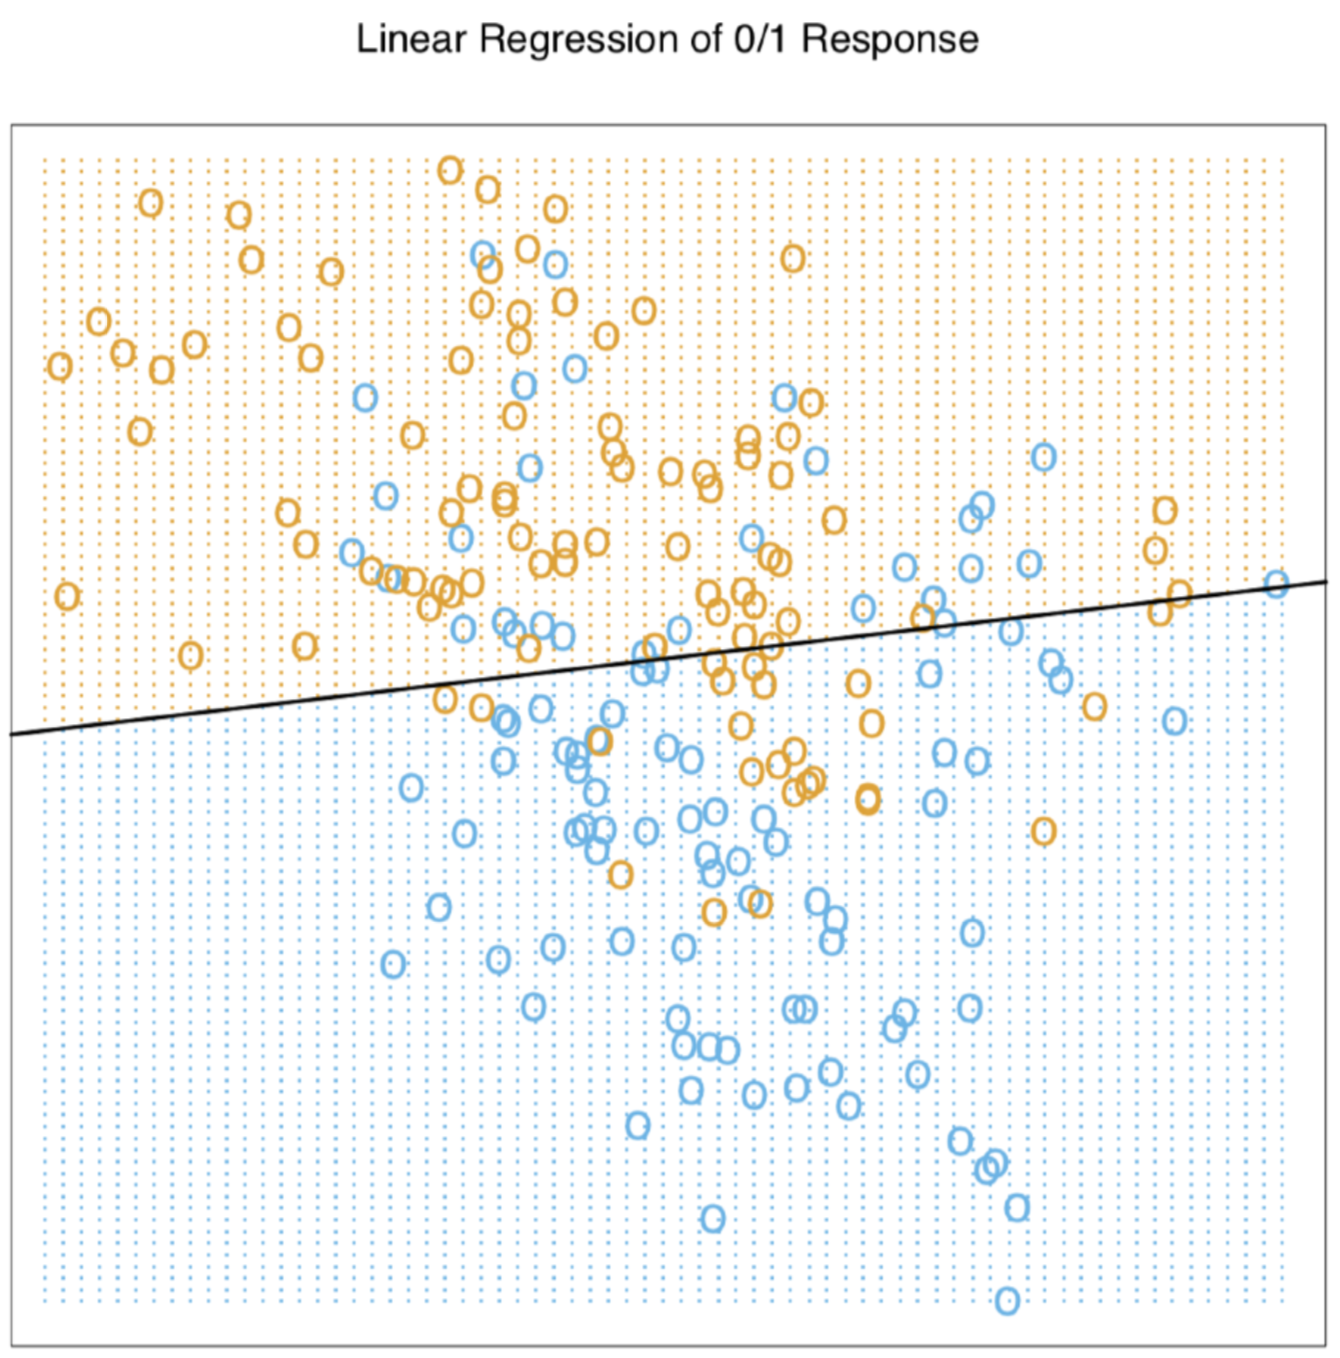
\includegraphics{./Figures/decboundary2D1.png}
    \caption{A classification example in two dimensions. The classes are coded
        as a binary variable (blue = 0, orange = 1), and then fit by linear
        regression. The line is the decision boundary, defined by
        $x^T \hat \beta = \half$ drawn as a black line. The orange shaded region
        denotes that part of input space classified as orange ($k=1$), while the
        blue region is classified as blue ($k=0$).
    }
    \label{decboundary2D1}
\end{marginfigure}

This method works only if the data are linearly separable -- \ie if we can
separate them in two sets of data by an hyperplan, defining the decision
boundary. We can there define an error.

It is worth noting that among many, we cannot predict in advance which prediction
method would work, without looking at the data. In practical, no method would
separate perfectly the data. If we augment the dimension of the space, we can
consider other functions. For example, quadratic regression would usually give
better results than linear. However, the use of higher dimensions spaces may
present tradeoffs: if we add more parameters, the training error would be reduced
, but the variance may also rise.
The issue here is to find the correct level of compexity that can fit the data,
without overfitting it and that can be generalised.

Again we'll use a second class of methods. ability to solve different issues.
fig 8 for example (marginfigure)

If we add to these data another class, for example $y=0,1,2$. There is now no
classical order between the values and the linear regression cannot be computed
on the three sets in one time. We have to split the data between two classes and
to find two decisions boundaries that split the three classes.

This was a very naive approach. Let's start again with $p=1$. Let's add more blue
squares at higher abscissa. This is presented in figure \ref{supvlearn7}


\begin{figure}
    \TODO
    \caption{Representation of a dataset with blue dots indexed as 0 and red
        dots indexed as 1. A linear regression can be plotted on these data
    }
    \label{supvlearn7}
\end{figure}

Here, we added data far enough to put the blue squares in another category.

The linear regression can be written as:

\begin{equation}
    \min_\beta \frac{1}{N} \sum_i (y_i - \beta x_i)^2
\end{equation}

We can see clearly that it is more convenient to work with more symmetric data.
Here we can define the error $\varepsilon_i$ for the $i$ index.

\begin{equation}
    \varepsilon_i = (y_i - \beta x_i)^2.
\end{equation}

For the $K=2$ problem, we can pose:

$k_i = \pm 1 bd$ if $\hat \beta x >0 => +1$
$if \hat \beta x<0 => -1$

What matters here is wether the quantity $\hat y = \hat \beta x$ has the correct
sign or not.

\begin{equation}
    L(\beta) = \frac{1}{N} \sum_i \max(0, -y_i\beta^T x_i)
\end{equation}

Here again, the idea is that when $\beta x$ is of the same sign as $y$, the
maximum is zero, and the error is zero. This is called hinge regression.

The idea of the problem is gradient descent, that as a smoother version, called
logistic regression.

the idea is to replace this version
fig 10.
\begin{equation}
    L(\beta) = \nth \sumin \ln (1+e^{-y_i \beta^T x_i} )
\end{equation}

he tries to minimise the error, and the split value with  that logistic regression.

we can also arrive to similar results by chosing different approaches.
this is connected to the kind of operations that are done in neural networks.
we will see this later on.

instead of taking the reflection y to be k, it's easier to consider y to be
a probability. it makes here much more sense to make a linear regression.
a probabilistic model, in which I want to describe the probability, given some data.
parameter $\omega$: weight, standard notation in neural networks, whereas $\beta$ is
much more used in classical regression/statistical learning models.

\begin{equation}
    P(k=1 | x,\omega)
\end{equation}

\begin{eqnarray}
    P(k=1|x,\omega ) & >  P(k=-1|x,\omega) & => \hat k = 1 \\
    & <      &  => \hat k = -1
\end{eqnarray}


if we are considering the log of the proabilities:
\begin{eqnarray}
    \ln \frac{P(k=1|x,\omega)}{P(k=-1|x,\omega)} & = & \omega^T x\\
    & = &  \sum_{j=1}^P \omega_j x_j (+\omega_0)
\end{eqnarray}


I don't have to always write $+\omega_0$, for convenience, just changes in the
problem that have no influence.

In general, I want to define a more relevant model.

Let's call:
\begin{equation}
    y=P(k=1|x,\omega)
\end{equation}
\begin{equation}
    \ln (\frac{y}{1-y}) = \omega^T x
\end{equation}

\begin{equation}
    \frac{y}{1-y} = \exp (\omega^T x)
\end{equation}

thus
\begin{equation}
    y = e^{\omega^T x} (1-y)
\end{equation}

therefore
\begin{equation}
    y(1+e^{\omega^T x}) = e^{\omega^T x}
\end{equation}

\begin{equation}
    y = \frac{e^{\omega^T x}}{1+e^{\omega^Tx}} = \frac{1}{1+e^{-\omega^T x}}
\end{equation}

\begin{equation}
    P(k|x,\omega) = \frac{1}{1+e^{-k\omega^T x}}
\end{equation}


\begin{equation}
    \mathcal{L}(\omega) = \frac{1}{N} \sum_i \ln P(k_i |x_i,\omega) MLE
\end{equation}

if i replace P by its form:

\begin{equation}
    \mathcal{L}(\omega) = - \frac{1}{N} \sum_i \ln (1 + e^{-k_i \omega^T x_i})
\end{equation}

Essentially, the idea was to apply the maximum likelihood. I had to make 
hypothesis on the general form of the model. Once I do this, I
end up with this function. The different with the one above:  minus sign.
not surprising: a likelihood we want to maximise, and not error we want to
minimize.

\begin{equation}
    \max_\omega \mathcal{L}(\omega) <=> \min_\beta L(\beta)
\end{equation}

in neural networks,

fig11

\begin{equation}
    u = \sum_{j=1}^p \omega_j x_j = \omega^T x 
\end{equation}
is called the activation.

several inputs, and one output based on this.
if $u>0$, then I have output $y=1$.
if $u<0$, then $y=0$.

in the context of neural networks, people prefer work with 0 and 1 rather than
$\pm 1$.

neuron is a classifier

fig11

\begin{equation}
    y = \phi (u)
\end{equation}

\begin{equation}
    \phi (u) = \frac{1}{1+e^{-u}}
\end{equation}

essentially, what we do, is considering the different inputs with different
weights.
At the end, we will end with more complex classifier models. this one is very
elementary.
there are very simple algorithms, like the gradient descent.


let's start again with the log likelihood:

\begin{eqnarray}
    \mathcal{L}(\omega) & = & \frac{1}{N} \sum_i (k_i \ln y_i + (1-k_i) \ln(1-y_i))\\
    & = & \frac{1}{N} \sum_i \ln P (k_i | x_i,\omega)
\end{eqnarray}

\begin{equation}
    y_i = P(k_i =1 |x,\omega)
\end{equation}

\begin{eqnarray}
    ln(P(\ldots)) & = y_i & \;\text{if}\; k_i = 1 \\
    & = 1-y_i & \;\text{if}\; k_i = 0
\end{eqnarray}

then we make the model by assuming:

\begin{equation}
    y_i = \phi (u_i) where u_i = \omega^T x_i = \sum_{j=1} \omega_j x_{ij}
\end{equation}

now, we want to compute the gradient.
it means to compute the derivative of the log likelihood:

\begin{equation}
    \frac{\partial \mathcal{L}}{\partial \omega_j} = \frac{1}{N} \sum_i (k_i \frac{1}{y_i} \frac{\partial y_i}{\partial\omega_j} - (1-k_i)
\frac{1}{1-y_i}) \frac{\partial y_i}{\partial \omega_j}
\end{equation}

with
\begin{equation}
    (\ldots) = \frac{ k_i (1-y_i) - (1-k_i)y_i}{y_i (1-y_i)} = \frac{k_i - y_i}{y_i (1-y_i)} 
\end{equation}


and \begin{equation}
    \frac{\partial y_i}{\partial \omega_j} = \phi'(u_i) \frac{\partial u_i}{\partial \omega_j} = \phi'(u_i) X_{ij}
\end{equation}


thus
\begin{equation}
    \frac{\partial \mathcal{L}}{\partial\omega_j} = \frac{1}{N} \sum_i \frac{\phi'(u_i)}{\phi(u_i) (1-\phi(u_i))} (k_i - y_i) x_{ij}
\end{equation}

\begin{equation}
    \phi (u) = \frac{1}{1+e^{-u}} => \frac{\phi''}{\phi (1-\phi)} = 1
\end{equation}

\begin{equation}
    \frac{\partial \mathcal{L}}{\partial \omega_j} = \frac{1}{N} \sum_i (k_i - y_i) x_{ij}
\end{equation}

for neural networks, the same idea as gradinet descent is called backpropagation
, but it is a bit more complicated.

fig 2.1: representation of classification.

support vector machine : SVM
problem formally attitred: 
\begin{equation}
    \min_\omega \sum_i \max(0,1-k_i \omega^T x_i ) + \lambda ||\omega||^2
\end{equation}

the exercise is trying to find what this function is doing.

standard linear regression: take care about the distance to the line.
when doing SVM: introducing some margin of errors.
this approach would count as an error even if we are on the right side of the
line but close to it.
we're not going to explain it here, but it looks very much linke the other frameworks.

another approach:
linear discriminant analysis (LDA)

we take a model (probabilistic), more gaussian like. the objective function is
to fit two classes by the gaussian, in such a way we maximise the distance
between the gaussians, and minimise the variance of the gaussians.
that can easily be done with linear algebra.

there are many other methods on the same lines.

Now we want to be able to adress the problem of non linear separability.
where the real boundary would be a circle.
in and out.

fig12

we can also do this locally.

it is called k-nearest neighbours

again, let's start with a batch of values:
fig13

we are given with a particular point, and say if it is red or blue.
what are the neighbours doing?

if $k=3$, i am looking at the three nearest points, and then take the colour of
the majority.

mathematically, it can be written as:

\begin{equation}
    \hat y(x)  = \frac{1}{k} \sum_{i\in N_k(x)} y_i
\end{equation}


$N_k(x)$ is the set of $k$ nearest neighbours to $x$

$y_i \in \{0,1\}$

Again, we can be in a situation described by fig 14.
we have, there, a decision boundary. i'm deciding what is the coulour of the
nearest points with that boundary.

fig 2.2 and 2.3. variations of K

now the question is: what should we take for K

$\frac{N}{k} \sim p$ : number of degrees of freedom.


fig 15

figure slide: 'selection of K': using 10,000 datapoints and tested with 200.

minimal training error if we take k=1. very complicated thing.
as we are taking larger and larger values of k, we are averaging and get more
errors, even in the training set.
if we have too few degrees of freedom, we are completely missing the structure
of data.
it is also not good if we have too many degrees of freedom.

15 is relatively well located in this area.
between 20 and 10, there's not that much difference, maybe 10 is better
because it uses less resources.
we have to pick the right model, and there are models of different levels of
complexity.
different values of k that can be used.

there is nothing into this algorithm, but also nothing trivial in finding the right datapoints.

there are many variations along this method.
in this example, we are taking the same density of points, everywhere. but if I take any point, it doesn't mean anything to take just three points
randomly.
we may take into account the distance between the points.
essentially, we would average around the point that are close to the considered
point. more generally, we can do it with a hard cutoff close/far or smooth
cutoffs.

\begin{equation}
    \hat y(x) = \frac{\sum_i K_\lambda (x,x_i)y_i}{\sum_i k_\lambda (x,x_i)}
\end{equation}

\begin{equation}
    K_\lambda (x,x_i) = \frac{1}{\lambda} e^{-\frac{||x-x'||^2}{2\lambda}}
\end{equation}

or $K_\lambda (x,x_i) = 1$ if $||x-x'||<\lambda$, 0 otherwise.

kernel methods also posisble.
if we do this, it is also a case where we have one parameter: $\lambda$. It plays
the same role.
big lambda: averaging a lot.
we would reduce the variance, but with a too large bias.
in the opposite: reduce the bias would end in a too large variance.

again, there are variety of methods that can be used. one way to see this
problem of classification is to fit a function.
let's say, zero for orange points, 1 for blue points.

At one dimension, we would have
fig 16.

maybe there could be errorsa

the thing is that we may smooth all those functinos.
we may think about these problems as fitting problems. correcting locally
the errors of the functions.

kernel method smoothing, to locally have something smoother.
what these things are doing is similar to the problem of smoothly inferring a
function from just any perfect observation.

This is very simple, but the problem is that none of those things are working
for big data. issue of classifying dogs and cats.

If we go in any of those methods, there is no way we can succeed. Several
problems, the greatest is a geometrical one:
the curse of dimensionality.

essentially, it has to do with all the assumption we have about neighbourhoods
are false when we are working with high dimensional spaces.

example in 2D in fig 17.

volume is scaling as power p of the radius. $V = \alpha_p r^p$.

If we look at $\frac{V}{V_{tot}} = \left( \frac{r}{r_{tot}} \right)^p$

then we have 

\begin{equation}
    \frac{r}{r_{tot}} = \left( \frac{V}{V_{tot}} \right)^{1/p}
\end{equation}


If the ratio $\frac{V}{V_{tot}} = 0.01$.
if we take something like p=10, we'll see that $\frac{r}{r_{tot}} = 0.6$.

if we want to cover even a very small fraction of the volume, we have to go very
far from the point.
ridiculous amount of the volume.
the problem of scaling with the radius is not interesting.
in high dimensional spaces, all the volume is close to the centre.

to cover a small fraction of the volume, we have to go very far.

All the ideas of closest neighhbourgs cannot be used in high dimensionality
spaces.

we can also reduce the dimensionality of the data. that is the first approach
with this problem.
solutions:
\begin{itemize}
    \item reduce dimensionality -> PCA (unsupervised)
    \item representation, that has to do with what kind of space we are woking with. we have to imagine that we have all the pictures of cats and
        dogs, all put in the same place.
        something invariant with translation, rotation, etc. so this will be seen in another lecture, about neural networks. essentially, one
        class of netwkrs: convolutional, is based on this. chose the right space
        in which it is easy to chose the classification.
\end{itemize}

exam
In priciple, everything should be comprised in the lecture.
code it ourself. not using things already written. the game here is to write
ourself our own libraries. it is not very complicated, each question is just
a few lines of code.

with python: using the jupyter.
matlab: not sure it is doeable. livescripts.
write a report in which he can see the code. in a format he can actually work
the code.
minimal thing: write the code and display the figures.
this is a public problem, neither on the solutions presented on the internet is
good, we might think about it from ourselves.





\chapter{Unsupervised learning: dimensionality reduction, PCA, SVD}
\label{ch:unsupervised-1}

\section{Dimensionality reduction}

So far we've seen only supervised learning, relation between two variables
(x,y). essentially, the goal was generalization of a relation between x and y

Today, we're going to see a bit of unsupervised learning.
this time, we only have x, no y anymore.
the goal is to find a pattern. we want to understand the data. it is a more
difficult problem. we think about problems of images.
we only have the picture, and it is our task to find how to classify them, and
what are the common things between all the data.
training set, validation set, test set : can not be done anymore. it is part of
the reason it is more difficult.
however, many things in common.
in the supervised context, at the end, it comes to optimization of a function l
of parameters x,y, and hyperparameters $\theta$,$\lambda$.

\hat \theta = \arg \min l(x,y,\theta,\lambda).

other approach, very similar : present the problem as a problem of optimisation.
a more probabilistic one is: we assume $P(x|y,\teta,\lambda)$. we have a 
statistical model. We have to decide what kind of probabilistic model we chose,
and how to parametrise it. Very often, we can formulate it.
Then we find the maximum likelihood $\mathcal{L}$ that we have to maximise,
similar to the loss function $l$ that we had to minimise.


for unsupervised learning:
dimensional reduction.
then we'll see clustering
in the last lecture : some generative models.

Let's start with dimensional reduction.
Motivation to do this dimensional reduction.
problem of the curse of dimensionality.

general approach with high dimension data is to reduce the data to low dimension
data.
we start with the first method in dimensonal reduction :

\subsection{Principle component analysis, PCA}

Probably one of the most useful method. the first we can do if we have large
datasets.
As usual, we have some data:
$x_{ij}$ where $i = 1\dots N$ the number of data, $j= 1\dots p$ the dimension.
dimension $d < p$.

let's start with $d=1$. how I can project the data on a line:
Let's start with $p=2$. I want to reduce it to $d=1$

photo 1.
we are looking to find a direction that explains more of the variation.
along the yellow line: almost just noise.
red = principal direction that explains the data.

Let's formulate it as an optimization problem.

Like in the linear regression, I am looking at the line that minimises the
distances between the line.

\begin{equation}
    l(a,m,v) = \nth \sumin ||x_i - m - a_i v ||^2
\end{equation}
and we assume that $||v||^2 = 1$ .
we are looking at the parameters $a,m,v$ that minimise the function.
We have to find the value of the projection as well as the data.

I am going to differentiate versus all these parameters, and check what we'll
get.

First, let's write it as:
\begin{equation}
    l(a,m,v) = \nth \sumin (x_i - m - a_iv)^T(x_i - m - a_iv).
\end{equation}
with $x_i - m - a_i v)$ is of $p$ dimension.

Let's start with a:

\begin{eqnarray}
    \frac{\partial l}{\partial a_i} & = & \nth v^T (x_i - m - a_i v)\\
     & = & \nth (v^T (x_i - m) - a_i) = 0
 \end{eqnarray}
 Therefore $\hat a_i = v^T (x_i - m) = (x_i - m)^T v$.

\begin{eqnarray}
     \frac{\partial l}{\partial m} & = & \nth \sumin (x_i - m - a_i v)\\
     & = & \nth \sumin [(x_i - m) - v^T (x_i - m) v] = 0
\end{eqnarray}

Therefore $\hat m = \bar x = \nth \sumin x_i$. Then we are left with the most
difficult part: optimise with respect to $v$.

To simplify, let's renormalise the data and consider:
\begin{eqnarray}
    l(\hat a, v) & = & \nth \sumin (||x_i||^2 - 2 x_i^T a_i v + \hat a_i^2 v^T v)\\
     & = & \nth \sumin (||x_i||^2 - \hat a_i^2 )
\end{eqnarray}

The reason to do it is because $v^Tv = 1$ and $x_i^T a_i v = \hat a_i^2$.

Let's write: 

\begin{equation}
    \nth \sumin \hat a_i^2 = \nth \sumin (v^T x_i)^2 = \nth \sumin \sum_{j=1}^p \sum_{k=1}^p v_j x_{ij} v_k x_{ik} = v^T C v
\end{equation}
with $C = \nth X^T X$, or $C_{jk} = \nth \sumin x_{ij} x_{ik}$.

$C_{jk}$ is the covariance matrix. the quantity we have to maximise is related
to the covariance matrix. maximising the left term in the previous equation.

is equivalent to find the minimum of the right term.

Finally, what I have to do is to find
$$ \max_v v^T C v $$
with the constraint of $||v||^2 = 1 $.

then we have the lagrangian function : 
$L (v) = v^T C v - \lambda v^T v$

$\frac{\partial L}{\partial v} = 2 (Cv-\lambda v) = 0$.

$C \hat v = \lambda \hat v$

At the end, we need to solve the spectrum of the matrix.
the direction $v$ is just going to be an eigenvector of C.
we need to understand which eigenvector, which one we want.
we want to maximise $v^T C v$. If I replace $C v $ by $\lambda v$, it is just

\begin{equation}
    \hat v^T C \hat v = \lambda \hat v^T \hat v = \lambda
\end{equation}

that we want to maximise.

principal component P c = eigenvector with largest eigenvalue $\lambda$

Again, there are lots of calculation, but at the end, the recipee is simple.
Compute C, like of correlation between every dimension.
look at the eigenvector that corresppond to the largest eigenvalue.
and then projection of what we want as a data.

The goal is to go from p at $d=1$, and then to generalise for $d\geq 1$.
We would have to consider cases such as
\begin{equation}
    l(a,v) = \nth \sumin || x_i - \sum_{k=1}^d a_{ik} v_k ||^2
\end{equation}

with $v_k^T v_j = \delta_k^j$.

we have $v_1,\ldots,v_d$ top eigenvectors of $C = \nth X^T X$.
associated with the largest eigenvalues:
$\lambda_1 \geq \lambda_2 \geq \cdots \geq \lambda_d \geq \lambda_{d+1} \geq \cdots \geq \lambda_p$

If I use it with generic data:

figure 14.20: what we did before.

PCA, human genomes.
SNP : some bases along the genome that are different along individuals.

4 bases: ATGC, and $L\sim 10^9$. we are looking only at some SNP because there
we are able to find differences
then get inforamtion about polymorphism.

The data is $X_{ij}$: 1000 individuals, and then many other dimensions.
The data that we get is:
all the sequences of SNPs: N = 3e^3 and dimension of p.

here it is only unsupervised.
then we can try to find a y : associations between particular diseases and
polymorphism. but not the problem here.

Here: we just have the data and try to find what are the structure of the data.
all depends on what kind of data we are working with.
in this case, people realise that when we compare. what are the relation ships
between individuals, in relation with their genomes.
compute a big correlation matrix: this is what $C_{jk}$ is doing.
if we rotate a bit the data, we find something like the map of europe.
PCA and what we get as a result is a representation vs the geography.
origin of the person doesn't go in the definition of the principal component.
There is a link in the paper.

peple have applied such analysis in other datasets, to reconstruct the history
of migrations, etc. If we compute those data, we'll find the eigenvalues.

but to get this, we need to reduce the datasets of 1000 individuals where we
knew the origins (two parents coming from determined places).
and then.

generally, there are a few cleaning steps before having proper data.
That was a simple example.

$X_{ij}$, N samples, p dim.
let's compute:

$C_{jk} = \nth \sumin x_{ij}x_{ik}$
and from here, let's compute the top eigenvectors of the matrix
$v_1,\ldots,v_d$

let's define a matrix called S:
$S_{ab} = \frac{1}{p} \sum_{a=1}^p x_{aj} x_{bj}$ and from this one, we can get
$U_1, \ldots, U_d$.
From here, I decide: let's look at the correlations between these ones, and the
correlations between SNPs.

this is where the SVD, \ie the singular value decomposition is coming to the picture.

\subsection{Singular value decomposition}
This is telling us, that the fact 

So, SVD is going to tell us that the two matrixes have the same spectrum:
$\lamda_1 = \mu_1, \ldots, \lambda_d = \mu_d$.

mathematical theorem is to say: we have a matrix $X_{ij}$ of size $N\times p$.
It is always possible to find two matrixes so that we can write:
\begin{equation}
    X = U \Sigma V^T
\end{equation}
with $U^T U  = 1doublebarre$
$V^T V = 1doublebarre$.

with \sigma is diagonal with a spectrum of dimension d.
there is always a way to transform the basis in the input-output space in a way
we are only mapping one vector of the basis, with another one in the factor.

\begin{eqnarray}
    C & = & X^T X\\
    & = &  (V \Sigma^T U^T)(U \Sigma V^T)\\
    & = & V (\Sigma^T \Sigma) V^T
\end{eqnarray}
And if we do p times S, we got:

\begin{eqnarray}
    pS & = & XX^T\\
    & = & (U \Sigma V^T)(V \Sigma^T U^T)\\
    & = & U (\Sigma \Sigma^T) U^T
\end{eqnarray}

with $\Sigma \Sigma^T = \Sigma^T \Sigma = \sigma_k^2$.

By using this kind of SVD mapping, we can relate the similarities that we see
between individuals to correlations between SNPs.

still an unanswered question: what do we take for d ?

here, d=2 to see it in relevant dimension, but in general?
it is something like an hyperparameter. usually with supervised learning, we
know what to do.

here, with unsupervised, we may use the information contained in the \lambda.
data is only one-dimensional.

let's draw $\rho(\lambda)$. first part of the spectrum = conrol data, and then
we have a $\lambda_1$. In general, we can look a the quantity:
\begin{equation}
    \frac{ \sum_{j=1}^d \lambda_j}{\sum_{j=1}^p \lambda_j}
\end{equation}

that is the fraction of variance explained by the top dimension PCs.

the typical criterion is to use this ratio.
it gives an indication of how much dimension use.

it is an empirical  criterion.

let's come back to the stocks example. first lambda value: almost 50. very large
variation. first mode of variation is global changes, we can assume as
a first approximation that all the stocks are varying the same way. most of the
variation that are present in the matrix C is just noise.
this is what we see.
typical spectrum we get from high dimensional problems.

then we have a few eigenvalues that are lower. Something we typically do when we
analyse that kind of data.
something we can do is randomise the data. for example making permutation
between the data. standard approach: shuffle the data.
it gives us back the control value. we will still compute some correlation
matrix. still capture some spectrum. what is written by control.
reproduce the lower part of the spectrum.
the message here is just to say, this is a standard criterium.
when we have a high dimensional data, the fact is that if we sum all the red
eigenvalues, the one that are considered as signal, only 2\% of the signal.
we want to set appart the signal from the noise, given the fact that
with high dimensional data, we have a lot of sampling noise.

we are projecting in low dimensions. companies have time to co-vary. will be put
together. what would be the eigenvectors? what kind of information could we get 
by projecting those kind of data?

the first two are similar, the last two are similar. the reason is that they're 
coming from the same industry.

PCA\& RMT: the sectors of the companies are taken as eigenvectors.
there are peaks at some companies. here we get information of the economy.
Information about different structures of the microbium, etc.
compute covariance matrixes, or covariance vectors. a way to understand the data
.



\chapter{Unsupervised learning: clustering, K-means, hierarchical}
\label{ch:unsupervised-2}
Clustering


The idea is simple: we want to classify our x. there are two methods. one is 
called K-means clustering.
the other hierarchical clustering.

as usual, the way is to use  functions we want to maximise/minimise.
cluster 1, cluster 2.
we have to find the cluster by ourselves.
measure of similarity/dissymilarity between points.
let's define a distance $d_{ii'}$. let's take, for example, just the euclidian
distance.

\begin{equation}
    d_{ii'} = ||x_i - x_{i'}||^2
\end{equation}

\begin{equation}
    W(C) = \half \sum_{k=1}^K \sum_{(i,i') \in C_k^2} 
\end{equation}

with a partition of my points:
K = # clusters.

{1,\ldots,N} = C_1 \union \cdots \union C_k

C_k \inter C_l = ensemble vide

\begin{equation}
    \min_C W(C) = ?
\end{equation}

we are not going to give all the details of the calculation.

\begin{equation}
    T = \half \sumin \sum_{i'=1}^N d_{ii'} = W(C) + B(C)
\end{equation}
with B defined by:
\begin{equation}
    B(C) = \half \sum_{k=1}^K \sum_{i\in C_k ; i'\notin C_k} d_{ii'}
\end{equation}

and finding $\min_C W(C)$ is then equivalent to find $\max_C B(C)$.

warning, this only works for the euclidian distance !!!!!!!!


exercise: let's work with:

\begin{equation}
    W(C) = \sum_{k=1}^K N_k \sum_{i\in C_k} || x_i - \bar x_k ||^2
\end{equation}
with $\bar x_k = \frac{1}{N_k} \sum_{i\in C_k} x_i$.
and $N_k = #C_k$

\begin{equation}
    \bar x = \arg \min_m \sumin || x_i - m_k||^2 = \frac{1}{N_k} \sum_{i=1}^{N_k} x_i
\end{equation}

\begin{equation}
    \min_C \min_{m_1,\ldots,m_k} \sum_{k=1}^K N_k \sum_{i\in C_k} ||x_i - m_k||^2
\end{equation}





















\begin{equation}
    \bar x = \arg \min_m \sumin || x_i - m_k||^2 = \frac{1}{N_k} \sum_{i=1}^{N_k} x_i
\end{equation}

\begin{equation}
    \min_C \min_{m_1,\ldots,m_k} \sum_{k=1}^K N_k \sum_{i\in C_k} ||x_i - m_k||^2
\end{equation}

k mean clustering.
we are doing the minimisation. start initially either with m or c.
we are assuming that the mean of cluster one has a particular position, mean
of cluster two is elsewhere.

we have to compute it in diferent ways. there we redefine the clusters, and recompute the means.

figure. once we redefine the mean, we recompute the clusters, and then redoit
iteratively.

the best way is to start from different points.
if we end up with two different clusterings, we can say which one is better.

let's now introduce another standard algorithm of clustering

a way not to solve this problem of k.

hierarchical clustering -> agglomerative
                        -> divisive.

we start in the case we construct clustering, each point is a cluster.
Then we make a clustering, and start with N clusters. make n clusters,

the first cluster that makes sense to compute, is just the minimum distances,
and say the minimum distnace is just replaced by a cluter.
initially, we just take the minimum between all the terms. At the end, we have
points, but all the points are clusters.


group average:
\begin{equation}
    \frac{1}{|C||C'|} \sum_{i,i' \in C} d_{ii'}
\end{equation}

single linkage:
\begin{equation}
    \min_{i\in C, i' \in C'} d_{ii'}
\end{equation}

complete linkage
\begin{equation}
    \max_{i \in C, i' \in C'} d_{ii'}
\end{equation}

in this way, we would make a series of N clusters.
N \rightarrow N-1 \rightarrow  until 1.

simple way to represent the data: dendogram. raprticular representation as a tree. cf fig 14.13.

essentially ,the dedograms are different.

















\chapter{Neural networks, from single neuron to multilayer networks}
\label{ch:neural-networks}
9 apr 18

most of the reason why people are excited about machine learning is
what has been made possible with neural networks. it is mostly related to what
we already seen.

representation of real neuron, VS mathematical object.
inspiration from biology.
brain organised as a network of neurons. each of these neurons are a processor
of information. many dendrites on which action potential coming in.
then axon, transfer of information as action potential.

scheme.
$y=\phi (u)$
$u = \sum_{j=1}^p \omega_j x_j$
$x_0 =1$

first example when $\phi$ is linear. linear regression.
example:
$\phi(u) = u$.
$l(\omega) = \sumin (y_i - \phi(u_i))^2$
taking the sum of squares. $\phi(u_i) = \sum_{j=1}^p \omega_j x_j$.
linear regression, first example.

another example that we've seen: logistic regresion (for classification).

in this context, we took:
$\phi(u) = \frac{1}{1+e^{-u}}$.
the cost function can be written as:
$l(\omega) = - \sumin k_i \ln y_i + (1-k_i) \ln (1-y_i)$
$y_i = P(k_i = 1|\omega,x) = \frac{e^{\omega^T x}}{1+e^{\omega^T x}}$
it is what we presented a few pages ago.
$l(\omega)$ looks very much like an entropy.
$y_i$ looks like a Boltzman distribution with a two-states system.

$P(E) = \frac{e^-{\betaE}}{Z}$: real boltzman distribution. two energies
E1 and E2. $P(E=E_1) = \frac{e^{\betaE}}{e^{-\betaE_0 + e^{-\beta E_1}}} = \frac{1}{1+e^{\beta\Delta E}}$.

if $K\geq 2$,
soft-max :
$k_{im} = 1$ if $i$ is in class $m$.
$i \in {1,\ldots, N}$ $m \in {1,\ldots,K}$.

generalisation of the same formula when we have more than two states:
$P(k_m = 1|x,\omega) = \frac{e^{x^T\omega_m}}{\sum_{n=1}^K e^{x^T\omega_m}}$

$l(\omega) = -\sumin \sum_{m=1}^K (k_{im} \ln y_{im} + (1-k_{im})\ln (1-y_{im}))$.

to find the best parameter of this model, write the function: maximum likelihood
estimation (MLE). write:

$\mathcal{L} = \ln P(\cdots)$
to minimise: $l = - \mathcal{L}$.

standard approach to define a model that is defined in term of probabilities.
mainly to remind that we've already seen many examples on single neurons.
essentially this will be discused later with classification of images.

network of neurons, the last layer will convert the likelihood into probabilities.
what is the probability that it is a dog, a cat, etc.

many different non linear functions that can be used. we can see the sigmoids.
nowadays in neural networks, ReLU and Leary ReLU are mostly used.

Leaky ReLU: does not saturate at high U

$\phi(u) = 1 if u>0, 0 if u \leq 0$.
let's consider $p=2$, $\omega_1 = \omega_2 = -2$, $\omega_0 = 3$.
let's consider that $x_1$ and $x_2$ are binary values : 0 or 1.
and then that $u = 3-2(x_1+x_2)$.

Let's see what are the different options.

$x_2$ \ $x_1$   0   1
0               1   1
1               1   0

it is a NAND gate
it is a way whith which we can make logical combinations.
this framework is one particular type of neurons. If I can do this, I can do any
kind of computation.
if we are doing picture recognition, input = pixels, output = what it is.


try to do some optimisation, try to organise the NAND gates, to get the circuit
that is going to achieve the function that we want. The big thing is that 
we need an algorithm to get the perfect circuit, network. with gradient descent
we can do it.
we don't have to think too much about the connection.
There would be two components.
the weights themselves are parameters.

If I take something more smooth by playing with the weights, I can do any
calculation that I want.

\subsection{Multilayer feedforward network}

in general, we could imagine many neural networks.
we have to train the network.
very simple algorithm: called multilayer feedforward network. network organised 
in layers.
last layer : output, classification in classes : number K of outputs.
input layer : pixels for example.
and inbetween, many hidden layers. feedforward, because all the connections are from one layer to the next, all oriented in the same way.

another type:

\subsection{Backpropagation algorithm}
smart implementation of gradient descent.
we can start with a single layer.
we've already seen this gradient descent algorithm.

single layer:
$l(\omega) = \half \sumin \sum_{m=1}^K (y_{im} - \phi(u_{im}))^2$
$u_{im} = \omega_m^T x_i = \sum_{j=1}^p \omega_{mj}x_{ij}$

$\frac{\partial l}{\partial \omega_{mj}} = - \sumin (y_{im} - \phi (u_{im}) \phi'(u_{im}) \frac{\partial u_{im}}{\partial \omega_{mj}}$
 = $ - \sumin e_{im} x_{ij}$

gradient descent

$\omega_{mj} \leftarrow \omega_{mj} - \eta \frac{\partial l}{\partial \omega_{mj}} = \omega_{mj} - \eta \sumin e_{im} x_{ij}$

on line: $\omega_{mj} \leftarrow \omega_{mj} - \eta e_{im} x_{ij}$.

we're gonna do the same in the context of neural networks.

$l(\omega) = \half \sumin \sum_{m=1}^k (y_{im} - x_{im}^{(L)})^2$

given any input, I update the data, layer by layer. that is called forward 
propagation : $x^(0) \rigtarrow x^{(1)} \rightarrow \cdots \rightarrow x^{(L)}$

$x_{j_k}^{(k)} = \phi (u_{j_k}^{(k)})$.
$u_{j_k}^{(k)} = \sum_{j_{k-1}} \omega_{j_k j_{k-1}} x_{j_{k-1}}^{(k-1)}$

secondly, bacward propagation:
$e^{(L)} \rightarrow e^{(L-1)} \rightarrow \cdots \rightarrow e^{(1)}$

$e_{j_L}^{(L)} = - (y_{j_L}^{(L)} - x_{j_L}^{(L)}) \phi'(u_{j_L}^{(L)}$


$e_{j_{k-1}}^{(k-1)} = \phi'(u_{j_{k-1}}^{(k-1)} \sum_{j_k} \omega_{j_kj_{k-1}}^{(k)} e_{j_k}^{(k)}$

At the end, when we've done this forward an d backward, we have an update, that
is the gradient descent. just take the product of the erors:

$\omega_{ab}^{(n)} \leftarrow \omega_{ab}^{(n)} - \eta e_a^{(n)} x_b^{(n-1)}$

What we'll try to do is derive??? those equations.

$\frac{\partial l}{\partial \omega_{ab}^{(n)}} = - \sum_{j_L = 1}^N (y_{j_L} - \phi (u_{j_L})) \phi'(u_{j_L}) \frac{\partial u_{j_L}}{\partial
\omega_{ab}^{(n)}}$

let's redefine the indexes:
layer k.
index j for the neuron inside the layer.
then we have $x_j^{(k)} = \phi(u_{j_k}^{(k)})$.

$\frac{\partial l}{\partial \omega_{ab}^{(n)}} = \sum_{j_{L-1}} \frac{\partial x_{j_{L-1}}^{(L-1)}}{\partial \omega_{ab}^{(n)}} \sum_{j_L}
\omega_{j_Lj_{L-1}}^{(L)} e_{j_L}^{(L)}$

this is true for $k = L-1$ as shown:

$\frac{\partial l}{\partial \omega_{ab}^{(n)}} = \sum_{j_k} \frac{x_{j_k}^{(k)}}{\partial \omega_{ab}^{(n)}} \sum_{j_{k+1}}
\omega_{j_{k+1}j_k}^{(k+1)}e_{j_{k+1}}^{(k+1)}$

with $\frac{\pratial x_{j_k}^{(k)}}{\partial \omega_{ab}^{(n)}} = \delta_{j_k}^a x_b^{(k)} \phi'(u_{j_k}^{(k)}$.
for n = k,

frac(\dots) = $x_b^{(k)} \phi'(u_a^{(k)} ) \sum_{j_{k+1}} \omega_{j_{k+1}a}^{(k+1)} e_{j_{k+1}}^{(k+1)}$


example. recognition of digits. coming from US postal services.
10 classes.
as inputs, we need one neuron for each pixel. output: we used something like
soft max. at the end, once we have trained these networks, set the value of the
first layer based on the digits. 

this example to show that only 15 neurons in the hidden layer.
what is written is only the backpropagation algorithm. no hyper parameter.
split into training set, and test set. training set larger.
let's look at the website, start a very complicated code.
relatively simple, already does 95\% accuracy. state of the art:99.8\%, that is 
what human would do.
deep neural networks: much many layers.

more complicated network can perform to the level of human perfection.
current application:
- image recognition picture, convolution networks
- process sequences that means process speech, movies or text. slightly
different architecture.
bit of idea of what goes in the current neural networks. essentially, the basic 
architecture\dots..

in one particular application, convolution networks, \dots
idea before going into description.
different layers, image is the first.
we want a transformation of these data in such a way that at the end, we can
apply a soft-max. \ie take our points, and put together all the images that are similar. there's a problem of the distance between the images. if we
take the raw images, take all the pictures of cats/dogs together.
at the end, project our data.
somewhat there are some special properties of images. if we make a slight 
rotation of the image, it doesn't change the distances.
identify the edges in the picture.
at the end, we convert the image in a series of activation maps, by applying
many filters. question: what filter should I use.
we are going to train the filters to find the good value of the weight that
is going to identify the particular data in the image.



mostly done with labels???


now, come back to PCA.
principal component analysis. simplest but most powerful approach that can be
applied to data.
that is unsupervised.

as usual ,the data are:
$x_{ij}$, $i = 1, \ldots, N$, $j=1,\ldots, p$.
what we have to compute is the covariance matrix:
$C_{ij}$. we normalise at first the data by substracting the mean.

$x'_{ij} = x_{ij} - \nth \sum_{a=1}^N x_{aj}$

$x' = x - \bar{x}$
then

$x'' = \frac{x'}{\sigma(x')}$

therefore the matrix C is p times p dimension.
So we will compute:
$C_{jk} = \nth \sumin x_{ij} x_{ik}$. it is a correlation function.
we can write it as:

$C_{jk} = \overline{x_j x_k}$.
in general, we should avoid making loops for sums, and find ways to compute it
with linear algearba. in this case:
$C_{jk} = \nth X^TX$
the eigenvalues and eigenvectors are :
$v_1, v_2, \ldots$ associated with $\lambda_1 \geq \lambda_2 \geq \cdots$.
In general, we have a matrix V composed of the eigenvetors in the columns.

we can represent the data by plotting the data versus $v_1$ and $v_2$.
they are defined as a multiplicative constant. and then project the data.
interpretation of that kind of diagram.
each feature is contributing to the eigenvectors. we have to think of them as
modes.
if we look back at the examples given by financial data, we are correlating the return of our stocks. When we have two companies that are behaving in
similar ways.










\chapter{Physics of machine learning, statistical mechanics of machine learning, applications}
\label{ch:physics}

application of physics ideas to this field.



\end{document}
